\documentclass[twoside]{book}

% Packages required by doxygen
\usepackage{fixltx2e}
\usepackage{calc}
\usepackage{doxygen}
\usepackage[export]{adjustbox} % also loads graphicx
\usepackage{graphicx}
\usepackage[utf8]{inputenc}
\usepackage{makeidx}
\usepackage{multicol}
\usepackage{multirow}
\PassOptionsToPackage{warn}{textcomp}
\usepackage{textcomp}
\usepackage[nointegrals]{wasysym}
\usepackage[table]{xcolor}

% Font selection
\usepackage[T1]{fontenc}
\usepackage[scaled=.90]{helvet}
\usepackage{courier}
\usepackage{amssymb}
\usepackage{sectsty}
\renewcommand{\familydefault}{\sfdefault}
\allsectionsfont{%
  \fontseries{bc}\selectfont%
  \color{darkgray}%
}
\renewcommand{\DoxyLabelFont}{%
  \fontseries{bc}\selectfont%
  \color{darkgray}%
}
\newcommand{\+}{\discretionary{\mbox{\scriptsize$\hookleftarrow$}}{}{}}

% Page & text layout
\usepackage{geometry}
\geometry{%
  a4paper,%
  top=2.5cm,%
  bottom=2.5cm,%
  left=2.5cm,%
  right=2.5cm%
}
\tolerance=750
\hfuzz=15pt
\hbadness=750
\setlength{\emergencystretch}{15pt}
\setlength{\parindent}{0cm}
\setlength{\parskip}{3ex plus 2ex minus 2ex}
\makeatletter
\renewcommand{\paragraph}{%
  \@startsection{paragraph}{4}{0ex}{-1.0ex}{1.0ex}{%
    \normalfont\normalsize\bfseries\SS@parafont%
  }%
}
\renewcommand{\subparagraph}{%
  \@startsection{subparagraph}{5}{0ex}{-1.0ex}{1.0ex}{%
    \normalfont\normalsize\bfseries\SS@subparafont%
  }%
}
\makeatother

% Headers & footers
\usepackage{fancyhdr}
\pagestyle{fancyplain}
\fancyhead[LE]{\fancyplain{}{\bfseries\thepage}}
\fancyhead[CE]{\fancyplain{}{}}
\fancyhead[RE]{\fancyplain{}{\bfseries\leftmark}}
\fancyhead[LO]{\fancyplain{}{\bfseries\rightmark}}
\fancyhead[CO]{\fancyplain{}{}}
\fancyhead[RO]{\fancyplain{}{\bfseries\thepage}}
\fancyfoot[LE]{\fancyplain{}{}}
\fancyfoot[CE]{\fancyplain{}{}}
\fancyfoot[RE]{\fancyplain{}{\bfseries\scriptsize Generated by Doxygen }}
\fancyfoot[LO]{\fancyplain{}{\bfseries\scriptsize Generated by Doxygen }}
\fancyfoot[CO]{\fancyplain{}{}}
\fancyfoot[RO]{\fancyplain{}{}}
\renewcommand{\footrulewidth}{0.4pt}
\renewcommand{\chaptermark}[1]{%
  \markboth{#1}{}%
}
\renewcommand{\sectionmark}[1]{%
  \markright{\thesection\ #1}%
}

% Indices & bibliography
\usepackage{natbib}
\usepackage[titles]{tocloft}
\setcounter{tocdepth}{3}
\setcounter{secnumdepth}{5}
\makeindex

% Hyperlinks (required, but should be loaded last)
\usepackage{ifpdf}
\ifpdf
  \usepackage[pdftex,pagebackref=true]{hyperref}
\else
  \usepackage[ps2pdf,pagebackref=true]{hyperref}
\fi
\hypersetup{%
  colorlinks=true,%
  linkcolor=blue,%
  citecolor=blue,%
  unicode%
}

% Custom commands
\newcommand{\clearemptydoublepage}{%
  \newpage{\pagestyle{empty}\cleardoublepage}%
}

\usepackage{caption}
\captionsetup{labelsep=space,justification=centering,font={bf},singlelinecheck=off,skip=4pt,position=top}

%===== C O N T E N T S =====

\begin{document}

% Titlepage & ToC
\hypersetup{pageanchor=false,
             bookmarksnumbered=true,
             pdfencoding=unicode
            }
\pagenumbering{alph}
\begin{titlepage}
\vspace*{7cm}
\begin{center}%
{\Large T\+C\+C\+Doxygen }\\
\vspace*{1cm}
{\large Generated by Doxygen 1.8.12}\\
\end{center}
\end{titlepage}
\clearemptydoublepage
\pagenumbering{roman}
\tableofcontents
\clearemptydoublepage
\pagenumbering{arabic}
\hypersetup{pageanchor=true}

%--- Begin generated contents ---
\chapter{Hierarchical Index}
\section{Class Hierarchy}
This inheritance list is sorted roughly, but not completely, alphabetically\+:\begin{DoxyCompactList}
\item \contentsline{section}{Stereo\+Utils\+:\+:Extras}{\pageref{class_stereo_utils_1_1_extras}}{}
\item Q\+Dialog\begin{DoxyCompactList}
\item \contentsline{section}{Set\+Stereo\+Params}{\pageref{class_set_stereo_params}}{}
\end{DoxyCompactList}
\item Q\+Main\+Window\begin{DoxyCompactList}
\item \contentsline{section}{Main\+Window}{\pageref{class_main_window}}{}
\end{DoxyCompactList}
\item \contentsline{section}{qt\+\_\+meta\+\_\+stringdata\+\_\+\+Main\+Window\+\_\+t}{\pageref{structqt__meta__stringdata___main_window__t}}{}
\item \contentsline{section}{qt\+\_\+meta\+\_\+stringdata\+\_\+\+Set\+Stereo\+Params\+\_\+t}{\pageref{structqt__meta__stringdata___set_stereo_params__t}}{}
\item Q\+Thread\begin{DoxyCompactList}
\item \contentsline{section}{Stereo\+Utils\+:\+:Sleeper}{\pageref{class_stereo_utils_1_1_sleeper}}{}
\end{DoxyCompactList}
\item \contentsline{section}{Reconstruction3D}{\pageref{class_reconstruction3_d}}{}
\item \contentsline{section}{Stereo\+Utils\+:\+:Resizer}{\pageref{class_stereo_utils_1_1_resizer}}{}
\item \contentsline{section}{Stereo\+Calib}{\pageref{class_stereo_calib}}{}
\item \contentsline{section}{Stereo\+Config}{\pageref{class_stereo_config}}{}
\begin{DoxyCompactList}
\item \contentsline{section}{Stereo\+Processor}{\pageref{class_stereo_processor}}{}
\end{DoxyCompactList}
\item \contentsline{section}{Stereo\+Diff}{\pageref{class_stereo_diff}}{}
\item \contentsline{section}{Stereo\+Disparity\+Map}{\pageref{class_stereo_disparity_map}}{}
\item \contentsline{section}{Stereo\+Flags}{\pageref{class_stereo_flags}}{}
\item \contentsline{section}{Stereo\+Input}{\pageref{class_stereo_input}}{}
\item \contentsline{section}{Stereo\+Morphology}{\pageref{class_stereo_morphology}}{}
\item \contentsline{section}{Stereo\+Rectify}{\pageref{class_stereo_rectify}}{}
\item \contentsline{section}{Stereo\+Utils\+:\+:Time}{\pageref{class_stereo_utils_1_1_time}}{}
\item \contentsline{section}{Track\+Object}{\pageref{class_track_object}}{}
\item \contentsline{section}{Ui\+\_\+\+Main\+Window}{\pageref{class_ui___main_window}}{}
\begin{DoxyCompactList}
\item \contentsline{section}{Ui\+:\+:Main\+Window}{\pageref{class_ui_1_1_main_window}}{}
\end{DoxyCompactList}
\item \contentsline{section}{Ui\+\_\+\+Set\+Stereo\+Params}{\pageref{class_ui___set_stereo_params}}{}
\begin{DoxyCompactList}
\item \contentsline{section}{Ui\+:\+:Set\+Stereo\+Params}{\pageref{class_ui_1_1_set_stereo_params}}{}
\end{DoxyCompactList}
\end{DoxyCompactList}

\chapter{Class Index}
\section{Class List}
Here are the classes, structs, unions and interfaces with brief descriptions\+:\begin{DoxyCompactList}
\item\contentsline{section}{\hyperlink{class_stereo_utils_1_1_extras}{Stereo\+Utils\+::\+Extras} }{\pageref{class_stereo_utils_1_1_extras}}{}
\item\contentsline{section}{\hyperlink{class_ui_1_1_main_window}{Ui\+::\+Main\+Window} }{\pageref{class_ui_1_1_main_window}}{}
\item\contentsline{section}{\hyperlink{class_main_window}{Main\+Window} }{\pageref{class_main_window}}{}
\item\contentsline{section}{\hyperlink{structqt__meta__stringdata___main_window__t}{qt\+\_\+meta\+\_\+stringdata\+\_\+\+Main\+Window\+\_\+t} }{\pageref{structqt__meta__stringdata___main_window__t}}{}
\item\contentsline{section}{\hyperlink{structqt__meta__stringdata___set_stereo_params__t}{qt\+\_\+meta\+\_\+stringdata\+\_\+\+Set\+Stereo\+Params\+\_\+t} }{\pageref{structqt__meta__stringdata___set_stereo_params__t}}{}
\item\contentsline{section}{\hyperlink{class_reconstruction3_d}{Reconstruction3D} }{\pageref{class_reconstruction3_d}}{}
\item\contentsline{section}{\hyperlink{class_stereo_utils_1_1_resizer}{Stereo\+Utils\+::\+Resizer} }{\pageref{class_stereo_utils_1_1_resizer}}{}
\item\contentsline{section}{\hyperlink{class_ui_1_1_set_stereo_params}{Ui\+::\+Set\+Stereo\+Params} }{\pageref{class_ui_1_1_set_stereo_params}}{}
\item\contentsline{section}{\hyperlink{class_set_stereo_params}{Set\+Stereo\+Params} }{\pageref{class_set_stereo_params}}{}
\item\contentsline{section}{\hyperlink{class_stereo_utils_1_1_sleeper}{Stereo\+Utils\+::\+Sleeper} }{\pageref{class_stereo_utils_1_1_sleeper}}{}
\item\contentsline{section}{\hyperlink{class_stereo_calib}{Stereo\+Calib} }{\pageref{class_stereo_calib}}{}
\item\contentsline{section}{\hyperlink{class_stereo_config}{Stereo\+Config} }{\pageref{class_stereo_config}}{}
\item\contentsline{section}{\hyperlink{class_stereo_diff}{Stereo\+Diff} }{\pageref{class_stereo_diff}}{}
\item\contentsline{section}{\hyperlink{class_stereo_disparity_map}{Stereo\+Disparity\+Map} }{\pageref{class_stereo_disparity_map}}{}
\item\contentsline{section}{\hyperlink{class_stereo_flags}{Stereo\+Flags} }{\pageref{class_stereo_flags}}{}
\item\contentsline{section}{\hyperlink{class_stereo_input}{Stereo\+Input} }{\pageref{class_stereo_input}}{}
\item\contentsline{section}{\hyperlink{class_stereo_morphology}{Stereo\+Morphology} }{\pageref{class_stereo_morphology}}{}
\item\contentsline{section}{\hyperlink{class_stereo_processor}{Stereo\+Processor} }{\pageref{class_stereo_processor}}{}
\item\contentsline{section}{\hyperlink{class_stereo_rectify}{Stereo\+Rectify} }{\pageref{class_stereo_rectify}}{}
\item\contentsline{section}{\hyperlink{class_stereo_utils_1_1_time}{Stereo\+Utils\+::\+Time} }{\pageref{class_stereo_utils_1_1_time}}{}
\item\contentsline{section}{\hyperlink{class_track_object}{Track\+Object} }{\pageref{class_track_object}}{}
\item\contentsline{section}{\hyperlink{class_ui___main_window}{Ui\+\_\+\+Main\+Window} }{\pageref{class_ui___main_window}}{}
\item\contentsline{section}{\hyperlink{class_ui___set_stereo_params}{Ui\+\_\+\+Set\+Stereo\+Params} }{\pageref{class_ui___set_stereo_params}}{}
\end{DoxyCompactList}

\chapter{Class Documentation}
\hypertarget{class_stereo_utils_1_1_extras}{}\section{Stereo\+Utils\+:\+:Extras Class Reference}
\label{class_stereo_utils_1_1_extras}\index{Stereo\+Utils\+::\+Extras@{Stereo\+Utils\+::\+Extras}}
\subsection*{Public Member Functions}
\begin{DoxyCompactItemize}
\item 
void {\bfseries contrast\+\_\+and\+\_\+brightness} (Mat \&left, Mat \&right, float alpha, float beta)\hypertarget{class_stereo_utils_1_1_extras_a6cefe41a723177e28963a6e5321dfa8f}{}\label{class_stereo_utils_1_1_extras_a6cefe41a723177e28963a6e5321dfa8f}

\item 
void {\bfseries write\+Mat\+To\+File} (Mat \&m, const char $\ast$filename)\hypertarget{class_stereo_utils_1_1_extras_a28415b181f246a77a5529019d99dfaab}{}\label{class_stereo_utils_1_1_extras_a28415b181f246a77a5529019d99dfaab}

\end{DoxyCompactItemize}
\subsection*{Static Public Member Functions}
\begin{DoxyCompactItemize}
\item 
static void \hyperlink{class_stereo_utils_1_1_extras_a94c111c1dec53fc39c24f42d26e98815}{calculate\+Hist} (Mat \&src, const string hist\+Name)
\item 
static string {\bfseries int\+To\+String} (int number)\hypertarget{class_stereo_utils_1_1_extras_a9d9937dd742a906f8ecd6bfad9123a00}{}\label{class_stereo_utils_1_1_extras_a9d9937dd742a906f8ecd6bfad9123a00}

\end{DoxyCompactItemize}


\subsection{Member Function Documentation}
\index{Stereo\+Utils\+::\+Extras@{Stereo\+Utils\+::\+Extras}!calculate\+Hist@{calculate\+Hist}}
\index{calculate\+Hist@{calculate\+Hist}!Stereo\+Utils\+::\+Extras@{Stereo\+Utils\+::\+Extras}}
\subsubsection[{\texorpdfstring{calculate\+Hist(\+Mat \&src, const string hist\+Name)}{calculateHist(Mat \&src, const string histName)}}]{\setlength{\rightskip}{0pt plus 5cm}void Stereo\+Utils\+::\+Extras\+::calculate\+Hist (
\begin{DoxyParamCaption}
\item[{Mat \&}]{src, }
\item[{const string}]{hist\+Name}
\end{DoxyParamCaption}
)\hspace{0.3cm}{\ttfamily [static]}}\hypertarget{class_stereo_utils_1_1_extras_a94c111c1dec53fc39c24f42d26e98815}{}\label{class_stereo_utils_1_1_extras_a94c111c1dec53fc39c24f42d26e98815}
Compute the histograms\+:

Compute the histograms\+: 

The documentation for this class was generated from the following files\+:\begin{DoxyCompactItemize}
\item 
inc/Stereo\+Utils.\+h\item 
src/Stereo\+Utils.\+cpp\end{DoxyCompactItemize}

\hypertarget{class_ui_1_1_main_window}{}\section{Ui\+:\+:Main\+Window Class Reference}
\label{class_ui_1_1_main_window}\index{Ui\+::\+Main\+Window@{Ui\+::\+Main\+Window}}


Inheritance diagram for Ui\+:\+:Main\+Window\+:
\nopagebreak
\begin{figure}[H]
\begin{center}
\leavevmode
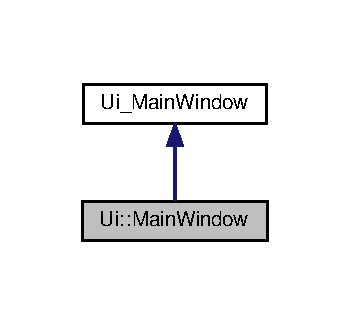
\includegraphics[width=168pt]{class_ui_1_1_main_window__inherit__graph}
\end{center}
\end{figure}


Collaboration diagram for Ui\+:\+:Main\+Window\+:
\nopagebreak
\begin{figure}[H]
\begin{center}
\leavevmode
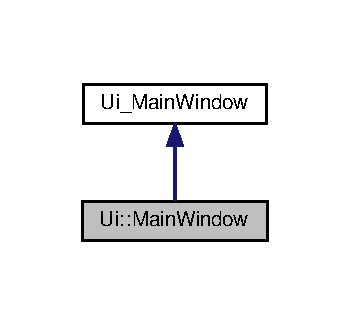
\includegraphics[width=168pt]{class_ui_1_1_main_window__coll__graph}
\end{center}
\end{figure}
\subsection*{Additional Inherited Members}


The documentation for this class was generated from the following file\+:\begin{DoxyCompactItemize}
\item 
tmp/moc/ui\+\_\+mainwindow.\+h\end{DoxyCompactItemize}

\hypertarget{class_main_window}{}\section{Main\+Window Class Reference}
\label{class_main_window}\index{Main\+Window@{Main\+Window}}


Inheritance diagram for Main\+Window\+:
\nopagebreak
\begin{figure}[H]
\begin{center}
\leavevmode
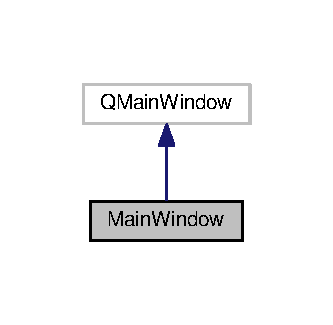
\includegraphics[width=160pt]{class_main_window__inherit__graph}
\end{center}
\end{figure}


Collaboration diagram for Main\+Window\+:
\nopagebreak
\begin{figure}[H]
\begin{center}
\leavevmode
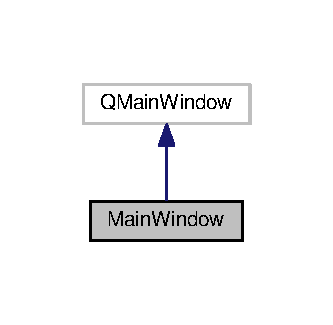
\includegraphics[width=160pt]{class_main_window__coll__graph}
\end{center}
\end{figure}
\subsection*{Public Types}
\begin{DoxyCompactItemize}
\item 
enum \{ {\bfseries L\+E\+F\+T\+\_\+\+W\+I\+N\+D\+OW}, 
{\bfseries R\+I\+G\+H\+T\+\_\+\+W\+I\+N\+D\+OW}
 \}\hypertarget{class_main_window_a0ee5fdf298d8f30b5e29418348ecaacf}{}\label{class_main_window_a0ee5fdf298d8f30b5e29418348ecaacf}

\end{DoxyCompactItemize}
\subsection*{Public Slots}
\begin{DoxyCompactItemize}
\item 
void {\bfseries stereo\+Vision\+Process\+\_\+\+Update\+G\+UI} ()\hypertarget{class_main_window_ab58219bc32f1d0a92b09c5eb33c4103b}{}\label{class_main_window_ab58219bc32f1d0a92b09c5eb33c4103b}

\end{DoxyCompactItemize}
\subsection*{Public Member Functions}
\begin{DoxyCompactItemize}
\item 
{\bfseries Main\+Window} (Q\+Widget $\ast$parent=0)\hypertarget{class_main_window_a8b244be8b7b7db1b08de2a2acb9409db}{}\label{class_main_window_a8b244be8b7b7db1b08de2a2acb9409db}

\item 
void {\bfseries ui\+Configuration} ()\hypertarget{class_main_window_a3527a1afb3344a1341fd80764713df2c}{}\label{class_main_window_a3527a1afb3344a1341fd80764713df2c}

\item 
void {\bfseries timer\+Configuration} ()\hypertarget{class_main_window_a50b34c2c0abf492a47587359634f0aa0}{}\label{class_main_window_a50b34c2c0abf492a47587359634f0aa0}

\item 
void {\bfseries setup\+Ui\+\_\+\+Custom} ()\hypertarget{class_main_window_aea0de3a599029b5f64f2a37dcebd8f86}{}\label{class_main_window_aea0de3a599029b5f64f2a37dcebd8f86}

\item 
void {\bfseries stereo\+Vision\+Process\+Init} ()\hypertarget{class_main_window_ad9655d307add03b591a644d3cbb60284}{}\label{class_main_window_ad9655d307add03b591a644d3cbb60284}

\item 
void {\bfseries print\+Help} ()\hypertarget{class_main_window_a64de1a7ba9c614b9b3bb86811f5e8bc2}{}\label{class_main_window_a64de1a7ba9c614b9b3bb86811f5e8bc2}

\item 
void {\bfseries open\+Stereo\+Source} (int input\+Num)\hypertarget{class_main_window_a9d9628939cd5f05b608835e85724163e}{}\label{class_main_window_a9d9628939cd5f05b608835e85724163e}

\item 
void {\bfseries delete\+Stereo\+Obj} ()\hypertarget{class_main_window_ae2ce9912561d8dc2973e96c46f57e7ba}{}\label{class_main_window_ae2ce9912561d8dc2973e96c46f57e7ba}

\item 
void {\bfseries pcl\+\_\+function} ()\hypertarget{class_main_window_a6c84072423be2737b33638670b2989b6}{}\label{class_main_window_a6c84072423be2737b33638670b2989b6}

\item 
void {\bfseries ui\+Text1} ()\hypertarget{class_main_window_af8d7ca80e733f594228f2bccdd083431}{}\label{class_main_window_af8d7ca80e733f594228f2bccdd083431}

\item 
void {\bfseries update\+Display\+Windows} ()\hypertarget{class_main_window_adf47e0731156f25c8f20f2a63b03cce6}{}\label{class_main_window_adf47e0731156f25c8f20f2a63b03cce6}

\item 
void {\bfseries put\+Image} (const Mat \&src, int window\+ID)\hypertarget{class_main_window_a1419aa870a37faeca4af58b6f00667cf}{}\label{class_main_window_a1419aa870a37faeca4af58b6f00667cf}

\item 
Q\+Image {\bfseries Mat2\+Q\+Image} (const Mat \&mat)\hypertarget{class_main_window_a42603613411483022b7b581948e5f418}{}\label{class_main_window_a42603613411483022b7b581948e5f418}

\end{DoxyCompactItemize}
\subsection*{Protected Member Functions}
\begin{DoxyCompactItemize}
\item 
void {\bfseries key\+Press\+Event} (Q\+Key\+Event $\ast$event)\hypertarget{class_main_window_a9c4f542263838b9ecd06eae839a42a34}{}\label{class_main_window_a9c4f542263838b9ecd06eae839a42a34}

\item 
void {\bfseries mouse\+Press\+Event} (Q\+Mouse\+Event $\ast$e)\hypertarget{class_main_window_aed2bdf63a7640182adfd5e959ea672d2}{}\label{class_main_window_aed2bdf63a7640182adfd5e959ea672d2}

\item 
void {\bfseries close\+Event} (Q\+Close\+Event $\ast$event)\hypertarget{class_main_window_a4e20a4a065fbb0e4d3532a45a0a91425}{}\label{class_main_window_a4e20a4a065fbb0e4d3532a45a0a91425}

\end{DoxyCompactItemize}


The documentation for this class was generated from the following files\+:\begin{DoxyCompactItemize}
\item 
inc/Main\+Window.\+h\item 
src/Main\+Window.\+cpp\end{DoxyCompactItemize}

\hypertarget{structqt__meta__stringdata___main_window__t}{}\section{qt\+\_\+meta\+\_\+stringdata\+\_\+\+Main\+Window\+\_\+t Struct Reference}
\label{structqt__meta__stringdata___main_window__t}\index{qt\+\_\+meta\+\_\+stringdata\+\_\+\+Main\+Window\+\_\+t@{qt\+\_\+meta\+\_\+stringdata\+\_\+\+Main\+Window\+\_\+t}}
\subsection*{Public Attributes}
\begin{DoxyCompactItemize}
\item 
Q\+Byte\+Array\+Data {\bfseries data} \mbox{[}17\mbox{]}\hypertarget{structqt__meta__stringdata___main_window__t_a392c18d82aabe0692a65dc6fac717b22}{}\label{structqt__meta__stringdata___main_window__t_a392c18d82aabe0692a65dc6fac717b22}

\item 
char {\bfseries stringdata} \mbox{[}431\mbox{]}\hypertarget{structqt__meta__stringdata___main_window__t_aed2e7da8c2facb2b317f017cc24cbbca}{}\label{structqt__meta__stringdata___main_window__t_aed2e7da8c2facb2b317f017cc24cbbca}

\end{DoxyCompactItemize}


The documentation for this struct was generated from the following file\+:\begin{DoxyCompactItemize}
\item 
tmp/moc/moc\+\_\+\+Main\+Window.\+cpp\end{DoxyCompactItemize}

\hypertarget{structqt__meta__stringdata___set_stereo_params__t}{}\section{qt\+\_\+meta\+\_\+stringdata\+\_\+\+Set\+Stereo\+Params\+\_\+t Struct Reference}
\label{structqt__meta__stringdata___set_stereo_params__t}\index{qt\+\_\+meta\+\_\+stringdata\+\_\+\+Set\+Stereo\+Params\+\_\+t@{qt\+\_\+meta\+\_\+stringdata\+\_\+\+Set\+Stereo\+Params\+\_\+t}}
\subsection*{Public Attributes}
\begin{DoxyCompactItemize}
\item 
Q\+Byte\+Array\+Data {\bfseries data} \mbox{[}25\mbox{]}\hypertarget{structqt__meta__stringdata___set_stereo_params__t_a25857eb28029d2512581336b539c537a}{}\label{structqt__meta__stringdata___set_stereo_params__t_a25857eb28029d2512581336b539c537a}

\item 
char {\bfseries stringdata} \mbox{[}842\mbox{]}\hypertarget{structqt__meta__stringdata___set_stereo_params__t_a5a88229ab18256cef34e6608d64a7850}{}\label{structqt__meta__stringdata___set_stereo_params__t_a5a88229ab18256cef34e6608d64a7850}

\end{DoxyCompactItemize}


The documentation for this struct was generated from the following files\+:\begin{DoxyCompactItemize}
\item 
tmp/moc/moc\+\_\+setstereoparams.\+cpp\item 
tmp/moc/moc\+\_\+\+Stereo\+Set\+Params\+Window.\+cpp\end{DoxyCompactItemize}

\hypertarget{class_reconstruction3_d}{}\section{Reconstruction3D Class Reference}
\label{class_reconstruction3_d}\index{Reconstruction3D@{Reconstruction3D}}
\subsection*{Public Member Functions}
\begin{DoxyCompactItemize}
\item 
void {\bfseries set\+View\+Point} (double x, double y, double z)\hypertarget{class_reconstruction3_d_a009c31d0f4ea78d4cc2caa3179085a59}{}\label{class_reconstruction3_d_a009c31d0f4ea78d4cc2caa3179085a59}

\item 
void {\bfseries set\+Look\+At\+Point} (double x, double y, double z)\hypertarget{class_reconstruction3_d_a0ab55481261b0a6f8c238a9944cb3377}{}\label{class_reconstruction3_d_a0ab55481261b0a6f8c238a9944cb3377}

\item 
void {\bfseries Point\+Cloud\+Init} (double baseline, bool is\+Sub)\hypertarget{class_reconstruction3_d_a3aa623f596ea3fbb9aec4e2bd8149778}{}\label{class_reconstruction3_d_a3aa623f596ea3fbb9aec4e2bd8149778}

\item 
void {\bfseries eular2rot} (double yaw, double pitch, double roll, Mat \&dest)\hypertarget{class_reconstruction3_d_a5c411c85a0c7bfe6d5d2bc6e06da324e}{}\label{class_reconstruction3_d_a5c411c85a0c7bfe6d5d2bc6e06da324e}

\item 
void {\bfseries lookat} (Point3d from, Point3d to, Mat \&destR)\hypertarget{class_reconstruction3_d_aa87d4367eee898a16c82cef4266e43ab}{}\label{class_reconstruction3_d_aa87d4367eee898a16c82cef4266e43ab}

\item 
void {\bfseries project\+Imagefrom\+X\+YZ} (Mat \&image, Mat \&destimage, Mat \&disp, Mat \&destdisp, Mat \&xyz, Mat \&R, Mat \&t, Mat \&K, Mat \&dist, bool is\+Sub)\hypertarget{class_reconstruction3_d_a771b752742d2a939b66b561946628df7}{}\label{class_reconstruction3_d_a771b752742d2a939b66b561946628df7}

\item 
void {\bfseries fill\+Occlusion} (Mat \&src, int invalidvalue, bool is\+Inv)\hypertarget{class_reconstruction3_d_a2b5edbc0e4ed41ed0bd4e3bbb9aa46ae}{}\label{class_reconstruction3_d_a2b5edbc0e4ed41ed0bd4e3bbb9aa46ae}

\end{DoxyCompactItemize}
\subsection*{Static Public Member Functions}
\begin{DoxyCompactItemize}
\item 
{\footnotesize template$<$class T $>$ }\\static void {\bfseries project\+Imagefrom\+X\+Y\+Z\+\_\+} (Mat \&image, Mat \&destimage, Mat \&disp, Mat \&destdisp, Mat \&xyz, Mat \&R, Mat \&t, Mat \&K, Mat \&dist, Mat \&mask, bool is\+Sub)\hypertarget{class_reconstruction3_d_a0224a67026665053a6e73733c2cf8384}{}\label{class_reconstruction3_d_a0224a67026665053a6e73733c2cf8384}

\item 
{\footnotesize template$<$class T $>$ }\\static void {\bfseries fill\+Occlusion\+\_\+} (Mat \&src, T invalidvalue)\hypertarget{class_reconstruction3_d_af7400ace09cc0c4f6dd1a9cd3596b46c}{}\label{class_reconstruction3_d_af7400ace09cc0c4f6dd1a9cd3596b46c}

\item 
{\footnotesize template$<$class T $>$ }\\static void {\bfseries fill\+Occlusion\+Inv\+\_\+} (Mat \&src, T invalidvalue)\hypertarget{class_reconstruction3_d_a6222d1f7eaffb47789bf199fbf332bac}{}\label{class_reconstruction3_d_a6222d1f7eaffb47789bf199fbf332bac}

\end{DoxyCompactItemize}
\subsection*{Public Attributes}
\begin{DoxyCompactItemize}
\item 
Mat {\bfseries disp3\+Dviewer}\hypertarget{class_reconstruction3_d_ab2a2dea7c42277f492ca369a0d681e49}{}\label{class_reconstruction3_d_ab2a2dea7c42277f492ca369a0d681e49}

\item 
Mat {\bfseries disp3D}\hypertarget{class_reconstruction3_d_af9ce9c97b445a5fd8c262284d6ed6aee}{}\label{class_reconstruction3_d_af9ce9c97b445a5fd8c262284d6ed6aee}

\item 
Mat {\bfseries disp3\+D\+\_\+8U}\hypertarget{class_reconstruction3_d_a896f2d6a8f2de090fb327d64e7c7e011}{}\label{class_reconstruction3_d_a896f2d6a8f2de090fb327d64e7c7e011}

\item 
Mat {\bfseries disp3\+D\+\_\+\+B\+GR}\hypertarget{class_reconstruction3_d_acc370e95411f18c09d378c3f2329f246}{}\label{class_reconstruction3_d_acc370e95411f18c09d378c3f2329f246}

\item 
Point3d {\bfseries viewpoint}\hypertarget{class_reconstruction3_d_a1994dca14df6d422c5c26ba90348614f}{}\label{class_reconstruction3_d_a1994dca14df6d422c5c26ba90348614f}

\item 
Point3d {\bfseries lookatpoint}\hypertarget{class_reconstruction3_d_acb4dd7f64781294fda22b5b8c0dc4617}{}\label{class_reconstruction3_d_acb4dd7f64781294fda22b5b8c0dc4617}

\item 
Mat {\bfseries dist}\hypertarget{class_reconstruction3_d_a65036ce8c5e8339e344455c9791319f4}{}\label{class_reconstruction3_d_a65036ce8c5e8339e344455c9791319f4}

\item 
Mat {\bfseries Rotation}\hypertarget{class_reconstruction3_d_aaa29e57ad3d91a75e3851cb932749cf0}{}\label{class_reconstruction3_d_aaa29e57ad3d91a75e3851cb932749cf0}

\item 
Mat {\bfseries t}\hypertarget{class_reconstruction3_d_aed09f325136179447d9525f6cc9ef467}{}\label{class_reconstruction3_d_aed09f325136179447d9525f6cc9ef467}

\item 
Mat {\bfseries xyz}\hypertarget{class_reconstruction3_d_a49b7b052f6f77d90a07097f235cba985}{}\label{class_reconstruction3_d_a49b7b052f6f77d90a07097f235cba985}

\item 
Mat {\bfseries depth}\hypertarget{class_reconstruction3_d_a00af4dca9c1d488144ce23329ce66e99}{}\label{class_reconstruction3_d_a00af4dca9c1d488144ce23329ce66e99}

\item 
double {\bfseries step}\hypertarget{class_reconstruction3_d_a41852efe3e2a50a2e80c4d8dd4f77773}{}\label{class_reconstruction3_d_a41852efe3e2a50a2e80c4d8dd4f77773}

\item 
bool {\bfseries is\+Sub}\hypertarget{class_reconstruction3_d_a67df1a6fff82ecbd603eea2dc8bc6235}{}\label{class_reconstruction3_d_a67df1a6fff82ecbd603eea2dc8bc6235}

\end{DoxyCompactItemize}


The documentation for this class was generated from the following files\+:\begin{DoxyCompactItemize}
\item 
inc/Reconstruction3\+D.\+h\item 
src/Reconstruction3\+D.\+cpp\end{DoxyCompactItemize}

\hypertarget{class_stereo_utils_1_1_resizer}{}\section{Stereo\+Utils\+:\+:Resizer Class Reference}
\label{class_stereo_utils_1_1_resizer}\index{Stereo\+Utils\+::\+Resizer@{Stereo\+Utils\+::\+Resizer}}
\subsection*{Static Public Member Functions}
\begin{DoxyCompactItemize}
\item 
static void {\bfseries resize\+Frames} (Mat $\ast$frame1, Mat $\ast$frame2, Size resolution)\hypertarget{class_stereo_utils_1_1_resizer_a81ffa2df134e07b9f43da76a9002de24}{}\label{class_stereo_utils_1_1_resizer_a81ffa2df134e07b9f43da76a9002de24}

\item 
static void {\bfseries change\+Resolution} (Video\+Capture $\ast$capL, Video\+Capture $\ast$capR, Size resolution)\hypertarget{class_stereo_utils_1_1_resizer_a49c1a46a8ac96f3891b4568e6fb2c501}{}\label{class_stereo_utils_1_1_resizer_a49c1a46a8ac96f3891b4568e6fb2c501}

\end{DoxyCompactItemize}


The documentation for this class was generated from the following files\+:\begin{DoxyCompactItemize}
\item 
inc/Stereo\+Utils.\+h\item 
src/Stereo\+Utils.\+cpp\end{DoxyCompactItemize}

\hypertarget{class_ui_1_1_set_stereo_params}{}\section{Ui\+:\+:Set\+Stereo\+Params Class Reference}
\label{class_ui_1_1_set_stereo_params}\index{Ui\+::\+Set\+Stereo\+Params@{Ui\+::\+Set\+Stereo\+Params}}


Inheritance diagram for Ui\+:\+:Set\+Stereo\+Params\+:
\nopagebreak
\begin{figure}[H]
\begin{center}
\leavevmode
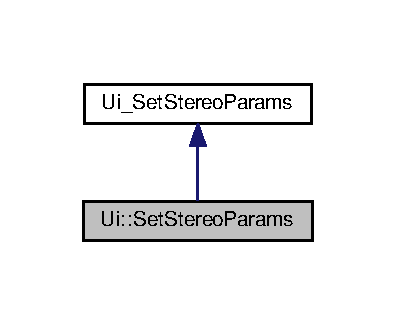
\includegraphics[width=190pt]{class_ui_1_1_set_stereo_params__inherit__graph}
\end{center}
\end{figure}


Collaboration diagram for Ui\+:\+:Set\+Stereo\+Params\+:
\nopagebreak
\begin{figure}[H]
\begin{center}
\leavevmode
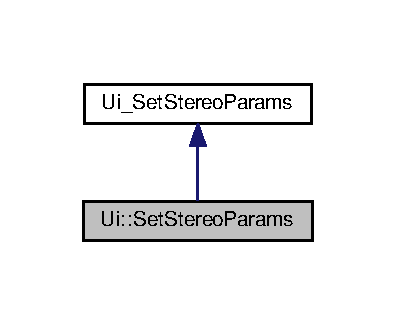
\includegraphics[width=190pt]{class_ui_1_1_set_stereo_params__coll__graph}
\end{center}
\end{figure}
\subsection*{Additional Inherited Members}


The documentation for this class was generated from the following file\+:\begin{DoxyCompactItemize}
\item 
tmp/moc/ui\+\_\+setstereoparams.\+h\end{DoxyCompactItemize}

\hypertarget{class_set_stereo_params}{}\section{Set\+Stereo\+Params Class Reference}
\label{class_set_stereo_params}\index{Set\+Stereo\+Params@{Set\+Stereo\+Params}}


Inheritance diagram for Set\+Stereo\+Params\+:
\nopagebreak
\begin{figure}[H]
\begin{center}
\leavevmode
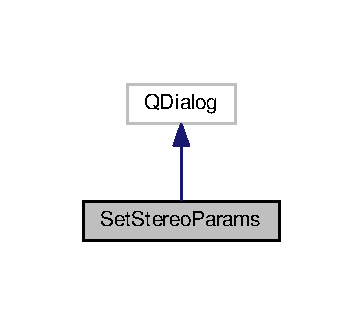
\includegraphics[width=174pt]{class_set_stereo_params__inherit__graph}
\end{center}
\end{figure}


Collaboration diagram for Set\+Stereo\+Params\+:
\nopagebreak
\begin{figure}[H]
\begin{center}
\leavevmode
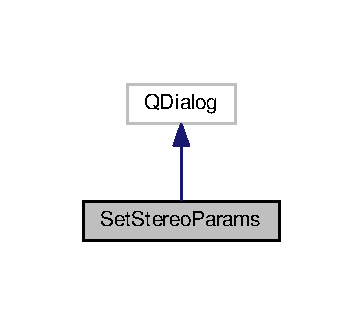
\includegraphics[width=174pt]{class_set_stereo_params__coll__graph}
\end{center}
\end{figure}
\subsection*{Public Member Functions}
\begin{DoxyCompactItemize}
\item 
{\bfseries Set\+Stereo\+Params} (Q\+Widget $\ast$parent=0, \hyperlink{class_stereo_processor}{Stereo\+Processor} $\ast$stereo=0)\hypertarget{class_set_stereo_params_aaf018e3767a36e75d67bff30054aeb13}{}\label{class_set_stereo_params_aaf018e3767a36e75d67bff30054aeb13}

\item 
void {\bfseries load\+Stereo\+Params\+Ui} (int pre\+Filter\+Size, int pre\+Filter\+Cap, int S\+A\+D\+Window\+Size, int min\+Disparity, int number\+Of\+Disparities, int texture\+Threshold, int uniqueness\+Ratio, int speckle\+Window\+Size, int speckle\+Range, int disp12\+Max\+Diff)\hypertarget{class_set_stereo_params_ae7d54e42d1b2ec75f0bf196beee5b002}{}\label{class_set_stereo_params_ae7d54e42d1b2ec75f0bf196beee5b002}

\end{DoxyCompactItemize}
\subsection*{Public Attributes}
\begin{DoxyCompactItemize}
\item 
bool {\bfseries is\+Already\+Showing}\hypertarget{class_set_stereo_params_a5f1883727db1c5b05ff573d1c66f0768}{}\label{class_set_stereo_params_a5f1883727db1c5b05ff573d1c66f0768}

\end{DoxyCompactItemize}


The documentation for this class was generated from the following files\+:\begin{DoxyCompactItemize}
\item 
inc/Stereo\+Set\+Params\+Window.\+h\item 
src/Stereo\+Set\+Params\+Window.\+cpp\end{DoxyCompactItemize}

\hypertarget{class_stereo_utils_1_1_sleeper}{}\section{Stereo\+Utils\+:\+:Sleeper Class Reference}
\label{class_stereo_utils_1_1_sleeper}\index{Stereo\+Utils\+::\+Sleeper@{Stereo\+Utils\+::\+Sleeper}}


Inheritance diagram for Stereo\+Utils\+:\+:Sleeper\+:
\nopagebreak
\begin{figure}[H]
\begin{center}
\leavevmode
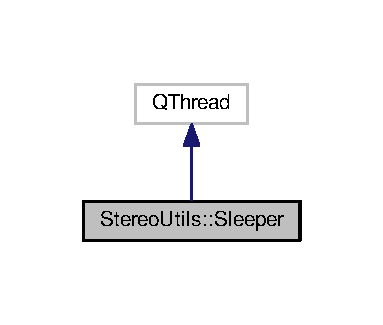
\includegraphics[width=184pt]{class_stereo_utils_1_1_sleeper__inherit__graph}
\end{center}
\end{figure}


Collaboration diagram for Stereo\+Utils\+:\+:Sleeper\+:
\nopagebreak
\begin{figure}[H]
\begin{center}
\leavevmode
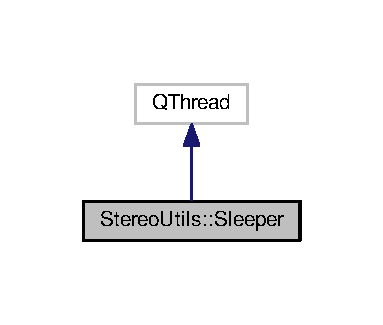
\includegraphics[width=184pt]{class_stereo_utils_1_1_sleeper__coll__graph}
\end{center}
\end{figure}
\subsection*{Static Public Member Functions}
\begin{DoxyCompactItemize}
\item 
static void {\bfseries usleep} (unsigned long usecs)\hypertarget{class_stereo_utils_1_1_sleeper_a72284b05dee22ca27a3a6c7d113b6508}{}\label{class_stereo_utils_1_1_sleeper_a72284b05dee22ca27a3a6c7d113b6508}

\item 
static void {\bfseries msleep} (unsigned long msecs)\hypertarget{class_stereo_utils_1_1_sleeper_ad0987958994e04889ee2b8bea3e809d6}{}\label{class_stereo_utils_1_1_sleeper_ad0987958994e04889ee2b8bea3e809d6}

\item 
static void {\bfseries sleep} (unsigned long secs)\hypertarget{class_stereo_utils_1_1_sleeper_a92c7a577a9435a7fd8cf431b08d03aef}{}\label{class_stereo_utils_1_1_sleeper_a92c7a577a9435a7fd8cf431b08d03aef}

\end{DoxyCompactItemize}


The documentation for this class was generated from the following file\+:\begin{DoxyCompactItemize}
\item 
inc/Stereo\+Utils.\+h\end{DoxyCompactItemize}

\hypertarget{class_stereo_calib}{}\section{Stereo\+Calib Class Reference}
\label{class_stereo_calib}\index{Stereo\+Calib@{Stereo\+Calib}}
\subsection*{Public Types}
\begin{DoxyCompactItemize}
\item 
enum \{ {\bfseries Video\+File}, 
{\bfseries Image\+File}
 \}\hypertarget{class_stereo_calib_abc54684cef2f45e2fc6858877d418b6c}{}\label{class_stereo_calib_abc54684cef2f45e2fc6858877d418b6c}

\end{DoxyCompactItemize}
\subsection*{Public Member Functions}
\begin{DoxyCompactItemize}
\item 
void {\bfseries read\+Calibration\+Files} ()\hypertarget{class_stereo_calib_a7525eb679794c618f5ddcda6037e154b}{}\label{class_stereo_calib_a7525eb679794c618f5ddcda6037e154b}

\item 
void {\bfseries read\+Intrinsics\+File} ()\hypertarget{class_stereo_calib_a971022931e4d6b3b48b766be554d03cc}{}\label{class_stereo_calib_a971022931e4d6b3b48b766be554d03cc}

\item 
void {\bfseries read\+Extrinsics\+File} ()\hypertarget{class_stereo_calib_a0c2402c9b8e192a2ec0f2005f223edec}{}\label{class_stereo_calib_a0c2402c9b8e192a2ec0f2005f223edec}

\item 
void {\bfseries read\+Q\+Matrix} ()\hypertarget{class_stereo_calib_a08b4daae32b930adc074f690f0af8f88}{}\label{class_stereo_calib_a08b4daae32b930adc074f690f0af8f88}

\item 
void {\bfseries calculate\+Q\+Matrix} ()\hypertarget{class_stereo_calib_afd8ad54a5076d898b567330185e6d3f3}{}\label{class_stereo_calib_afd8ad54a5076d898b567330185e6d3f3}

\item 
void {\bfseries create\+K\+Matrix} ()\hypertarget{class_stereo_calib_aea6e162e441033fad575cad449f43ecb}{}\label{class_stereo_calib_aea6e162e441033fad575cad449f43ecb}

\item 
void {\bfseries set\+Resolution} (int width, int height)\hypertarget{class_stereo_calib_a24699e443d80f5fdf3ec5503427ff129}{}\label{class_stereo_calib_a24699e443d80f5fdf3ec5503427ff129}

\item 
void {\bfseries set\+Resolution\+Desired} (int width, int height)\hypertarget{class_stereo_calib_aea0ba39cbf27b07d28ff4e5ae0913527}{}\label{class_stereo_calib_aea0ba39cbf27b07d28ff4e5ae0913527}

\item 
Size {\bfseries get\+Resolution} ()\hypertarget{class_stereo_calib_aa4d979e92c08c3ccd765b06c11348fba}{}\label{class_stereo_calib_aa4d979e92c08c3ccd765b06c11348fba}

\item 
Size {\bfseries get\+Resolution\+Desired} ()\hypertarget{class_stereo_calib_a8078af2c4898c07210b3bc8f599b105c}{}\label{class_stereo_calib_a8078af2c4898c07210b3bc8f599b105c}

\item 
int {\bfseries get\+Resolution\+\_\+width} ()\hypertarget{class_stereo_calib_a5a3bb4b2b3eff1b2c7386fccc7e0b9b6}{}\label{class_stereo_calib_a5a3bb4b2b3eff1b2c7386fccc7e0b9b6}

\item 
int {\bfseries get\+Resolution\+\_\+height} ()\hypertarget{class_stereo_calib_ad8e238d0b924a8708bd52bb62239e0c3}{}\label{class_stereo_calib_ad8e238d0b924a8708bd52bb62239e0c3}

\item 
int {\bfseries get\+Resolution\+Desired\+\_\+width} ()\hypertarget{class_stereo_calib_a7fa66ae1772dd4a6d78c71f0fd3573bf}{}\label{class_stereo_calib_a7fa66ae1772dd4a6d78c71f0fd3573bf}

\item 
int {\bfseries get\+Resolution\+Desired\+\_\+height} ()\hypertarget{class_stereo_calib_a7a2a248a3cf2bf2ed15e3b1d2d88f7ad}{}\label{class_stereo_calib_a7a2a248a3cf2bf2ed15e3b1d2d88f7ad}

\end{DoxyCompactItemize}
\subsection*{Public Attributes}
\begin{DoxyCompactItemize}
\item 
string {\bfseries image\+L\+\_\+\+File\+Name}\hypertarget{class_stereo_calib_ab3170ca0cdb6d029819cb3ffb4ccbb5b}{}\label{class_stereo_calib_ab3170ca0cdb6d029819cb3ffb4ccbb5b}

\item 
string {\bfseries image\+R\+\_\+\+File\+Name}\hypertarget{class_stereo_calib_aa881b7be6b75603581c58557e71a5212}{}\label{class_stereo_calib_aa881b7be6b75603581c58557e71a5212}

\item 
string {\bfseries intrinsics\+File\+Name}\hypertarget{class_stereo_calib_a0de8ba0185de07f46378fcca016923a2}{}\label{class_stereo_calib_a0de8ba0185de07f46378fcca016923a2}

\item 
string {\bfseries extrinsics\+File\+Name}\hypertarget{class_stereo_calib_a477840f6804f140fccdc0af4eb820144}{}\label{class_stereo_calib_a477840f6804f140fccdc0af4eb820144}

\item 
string {\bfseries Qmatrix\+File\+Name}\hypertarget{class_stereo_calib_a417c313faa6f3aed0193fe023da8faf9}{}\label{class_stereo_calib_a417c313faa6f3aed0193fe023da8faf9}

\item 
enum Stereo\+Calib\+:: \{ ... \}  {\bfseries input\+Type}\hypertarget{class_stereo_calib_adf965991ec0d973fe7ceac3d62e45d98}{}\label{class_stereo_calib_adf965991ec0d973fe7ceac3d62e45d98}

\item 
bool {\bfseries need\+Calibration}\hypertarget{class_stereo_calib_a9eb8ec0523950dc79930ca6c4f8d769d}{}\label{class_stereo_calib_a9eb8ec0523950dc79930ca6c4f8d769d}

\item 
bool {\bfseries has\+Q\+Matrix}\hypertarget{class_stereo_calib_aef06d162b6f5638181de3d81a51680de}{}\label{class_stereo_calib_aef06d162b6f5638181de3d81a51680de}

\item 
string {\bfseries Stereo\+B\+M\+Config\+File\+Name}\hypertarget{class_stereo_calib_ad8c790edd320cc7c0c8d99f3290d9934}{}\label{class_stereo_calib_ad8c790edd320cc7c0c8d99f3290d9934}

\item 
string {\bfseries Stereo\+S\+G\+B\+M\+Config\+File\+Name}\hypertarget{class_stereo_calib_ab39bf50aa2351d803c4f0c3587bc8f85}{}\label{class_stereo_calib_ab39bf50aa2351d803c4f0c3587bc8f85}

\item 
string {\bfseries Stereo\+B\+M\+\_\+\+G\+P\+U\+Config\+File\+Name}\hypertarget{class_stereo_calib_a8a101f83f7c8658bdbc979cc7604da7c}{}\label{class_stereo_calib_a8a101f83f7c8658bdbc979cc7604da7c}

\item 
Point2d {\bfseries image\+Center}\hypertarget{class_stereo_calib_aeebd81b1fef9762b6171bb69a54b955e}{}\label{class_stereo_calib_aeebd81b1fef9762b6171bb69a54b955e}

\item 
Mat {\bfseries K}\hypertarget{class_stereo_calib_ad055d005c5506befd16edb185e21233d}{}\label{class_stereo_calib_ad055d005c5506befd16edb185e21233d}

\item 
Mat {\bfseries Q}\hypertarget{class_stereo_calib_ad8423000f1dde7e8f9d03770506eb01b}{}\label{class_stereo_calib_ad8423000f1dde7e8f9d03770506eb01b}

\item 
double {\bfseries focal\+Length}\hypertarget{class_stereo_calib_af47674c0bb306d01d03dc7a3d727dc08}{}\label{class_stereo_calib_af47674c0bb306d01d03dc7a3d727dc08}

\item 
double {\bfseries baseline}\hypertarget{class_stereo_calib_a0ae91099682d585e07dcb61e0fa629b4}{}\label{class_stereo_calib_a0ae91099682d585e07dcb61e0fa629b4}

\item 
Mat {\bfseries M1}\hypertarget{class_stereo_calib_ab93c232d69d78bdc7b1b485fb36207d7}{}\label{class_stereo_calib_ab93c232d69d78bdc7b1b485fb36207d7}

\item 
Mat {\bfseries D1}\hypertarget{class_stereo_calib_acf3a38c2a866f0b183aebec6139ef935}{}\label{class_stereo_calib_acf3a38c2a866f0b183aebec6139ef935}

\item 
Mat {\bfseries M2}\hypertarget{class_stereo_calib_a98aaed9d770345d1fe5c2a1eace17197}{}\label{class_stereo_calib_a98aaed9d770345d1fe5c2a1eace17197}

\item 
Mat {\bfseries D2}\hypertarget{class_stereo_calib_aa8adb526019c31b55acf4d5ae7070a1d}{}\label{class_stereo_calib_aa8adb526019c31b55acf4d5ae7070a1d}

\item 
Mat {\bfseries R}\hypertarget{class_stereo_calib_a7adef19579d6c9038559cec648e3fcfe}{}\label{class_stereo_calib_a7adef19579d6c9038559cec648e3fcfe}

\item 
Mat {\bfseries T}\hypertarget{class_stereo_calib_a8a691c626521ea41c641191aed961fef}{}\label{class_stereo_calib_a8a691c626521ea41c641191aed961fef}

\item 
Mat {\bfseries R1}\hypertarget{class_stereo_calib_a3d033e22e18823cd70293e1e15930bae}{}\label{class_stereo_calib_a3d033e22e18823cd70293e1e15930bae}

\item 
Mat {\bfseries P1}\hypertarget{class_stereo_calib_af5ebf388ee3dbf37e8ead9e97fd35edf}{}\label{class_stereo_calib_af5ebf388ee3dbf37e8ead9e97fd35edf}

\item 
Mat {\bfseries R2}\hypertarget{class_stereo_calib_abd3f37a1a9a35c52adbe712c76830638}{}\label{class_stereo_calib_abd3f37a1a9a35c52adbe712c76830638}

\item 
Mat {\bfseries P2}\hypertarget{class_stereo_calib_ae8704396ef9f76572c92f514af3a55a3}{}\label{class_stereo_calib_ae8704396ef9f76572c92f514af3a55a3}

\item 
Rect {\bfseries roi1}\hypertarget{class_stereo_calib_a7a2e42914c5e2690f1f3f8d22eb28c9c}{}\label{class_stereo_calib_a7a2e42914c5e2690f1f3f8d22eb28c9c}

\item 
Rect {\bfseries roi2}\hypertarget{class_stereo_calib_aa2a6d011851c59315217149cbe70c374}{}\label{class_stereo_calib_aa2a6d011851c59315217149cbe70c374}

\item 
bool {\bfseries is\+Kcreated}\hypertarget{class_stereo_calib_a780a6de79ba19e0dd1b51e1ccfb9dcd2}{}\label{class_stereo_calib_a780a6de79ba19e0dd1b51e1ccfb9dcd2}

\end{DoxyCompactItemize}


The documentation for this class was generated from the following files\+:\begin{DoxyCompactItemize}
\item 
inc/Stereo\+Calib.\+h\item 
src/Stereo\+Calib.\+cpp\end{DoxyCompactItemize}

\hypertarget{class_stereo_config}{}\section{Stereo\+Config Class Reference}
\label{class_stereo_config}\index{Stereo\+Config@{Stereo\+Config}}


Inheritance diagram for Stereo\+Config\+:
\nopagebreak
\begin{figure}[H]
\begin{center}
\leavevmode
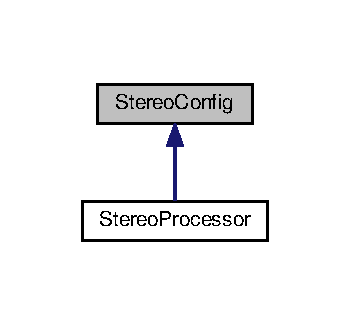
\includegraphics[width=168pt]{class_stereo_config__inherit__graph}
\end{center}
\end{figure}
\subsection*{Public Member Functions}
\begin{DoxyCompactItemize}
\item 
void {\bfseries show\+Config\+Values} ()\hypertarget{class_stereo_config_a6fe1655471974d26a20d362916132697}{}\label{class_stereo_config_a6fe1655471974d26a20d362916132697}

\end{DoxyCompactItemize}
\subsection*{Public Attributes}
\begin{DoxyCompactItemize}
\item 
string {\bfseries method\+Name}\hypertarget{class_stereo_config_ad307276f72bf2fbd0592437ce134d9b4}{}\label{class_stereo_config_ad307276f72bf2fbd0592437ce134d9b4}

\item 
int {\bfseries pre\+Filter\+Size}\hypertarget{class_stereo_config_a9a4278d21c09da39d7456a5977928c50}{}\label{class_stereo_config_a9a4278d21c09da39d7456a5977928c50}

\item 
int {\bfseries pre\+Filter\+Cap}\hypertarget{class_stereo_config_af6a5e6526165d701c448b591d3f0de43}{}\label{class_stereo_config_af6a5e6526165d701c448b591d3f0de43}

\item 
int {\bfseries S\+A\+D\+Window\+Size}\hypertarget{class_stereo_config_a9c877cdffa37e19840f4a18dc6a54f6d}{}\label{class_stereo_config_a9c877cdffa37e19840f4a18dc6a54f6d}

\item 
int {\bfseries min\+Disparity}\hypertarget{class_stereo_config_ad0897ddeb960edeb39a1fe735fa48390}{}\label{class_stereo_config_ad0897ddeb960edeb39a1fe735fa48390}

\item 
int {\bfseries number\+Of\+Disparities}\hypertarget{class_stereo_config_afa6a69b53d552a8acaefb440742eb5af}{}\label{class_stereo_config_afa6a69b53d552a8acaefb440742eb5af}

\item 
int {\bfseries texture\+Threshold}\hypertarget{class_stereo_config_a70bc91fd99847fb814bbc21deb436b3b}{}\label{class_stereo_config_a70bc91fd99847fb814bbc21deb436b3b}

\item 
int {\bfseries uniqueness\+Ratio}\hypertarget{class_stereo_config_a367ae211dc949080777958e67ad389d7}{}\label{class_stereo_config_a367ae211dc949080777958e67ad389d7}

\item 
int {\bfseries speckle\+Window\+Size}\hypertarget{class_stereo_config_ae37d8112b7ed2fd319121a03518dcedc}{}\label{class_stereo_config_ae37d8112b7ed2fd319121a03518dcedc}

\item 
int {\bfseries speckle\+Range}\hypertarget{class_stereo_config_af18849575709c1e7b073fa8660595188}{}\label{class_stereo_config_af18849575709c1e7b073fa8660595188}

\item 
int {\bfseries disp12\+Max\+Diff}\hypertarget{class_stereo_config_a041155ce140283dde736e3a3f4022c23}{}\label{class_stereo_config_a041155ce140283dde736e3a3f4022c23}

\end{DoxyCompactItemize}


The documentation for this class was generated from the following files\+:\begin{DoxyCompactItemize}
\item 
inc/Stereo\+Config.\+h\item 
src/Stereo\+Config.\+cpp\end{DoxyCompactItemize}

\hypertarget{class_stereo_diff}{}\section{Stereo\+Diff Class Reference}
\label{class_stereo_diff}\index{Stereo\+Diff@{Stereo\+Diff}}
\subsection*{Public Member Functions}
\begin{DoxyCompactItemize}
\item 
void {\bfseries create\+Diff\+Image} (Mat, Mat)\hypertarget{class_stereo_diff_afc5a133f69774c3299450672042cb102}{}\label{class_stereo_diff_afc5a133f69774c3299450672042cb102}

\item 
void {\bfseries create\+Res\+A\+ND} (Mat, Mat)\hypertarget{class_stereo_diff_a7631b179ab681be6e533d97d95d0968a}{}\label{class_stereo_diff_a7631b179ab681be6e533d97d95d0968a}

\item 
void {\bfseries convert\+To\+B\+GR} ()\hypertarget{class_stereo_diff_afe807062ba0099d50a424f888d1edeb2}{}\label{class_stereo_diff_afe807062ba0099d50a424f888d1edeb2}

\item 
void {\bfseries add\+Red\+Lines} ()\hypertarget{class_stereo_diff_a1e7272d98e86d4329d59873a63a5aecb}{}\label{class_stereo_diff_a1e7272d98e86d4329d59873a63a5aecb}

\end{DoxyCompactItemize}
\subsection*{Public Attributes}
\begin{DoxyCompactItemize}
\item 
bool {\bfseries Start\+Diff}\hypertarget{class_stereo_diff_acee17a3791ca92ad8b65cc12d6b08177}{}\label{class_stereo_diff_acee17a3791ca92ad8b65cc12d6b08177}

\item 
Mat {\bfseries diff\+Image}\hypertarget{class_stereo_diff_a652b54fb8337300919097a8b44097034}{}\label{class_stereo_diff_a652b54fb8337300919097a8b44097034}

\item 
Mat {\bfseries res\+\_\+\+A\+ND}\hypertarget{class_stereo_diff_a595f25af352ef8fa77ea110dd3ab1b43}{}\label{class_stereo_diff_a595f25af352ef8fa77ea110dd3ab1b43}

\item 
Mat {\bfseries imageL}\hypertarget{class_stereo_diff_a0ff31e2271dc9f2a2c97577798b0b5aa}{}\label{class_stereo_diff_a0ff31e2271dc9f2a2c97577798b0b5aa}

\item 
Mat {\bfseries res\+\_\+\+A\+N\+D\+\_\+\+B\+GR}\hypertarget{class_stereo_diff_a870bc6fcf520458156093088e60d4ce3}{}\label{class_stereo_diff_a870bc6fcf520458156093088e60d4ce3}

\item 
Mat {\bfseries res\+\_\+\+A\+N\+D\+\_\+\+B\+G\+R\+\_\+channels} \mbox{[}3\mbox{]}\hypertarget{class_stereo_diff_a314bc381fd8e199747171714788ce3a8}{}\label{class_stereo_diff_a314bc381fd8e199747171714788ce3a8}

\item 
double {\bfseries alpha}\hypertarget{class_stereo_diff_a6bccf2369ffd1af72befc554fd7a558b}{}\label{class_stereo_diff_a6bccf2369ffd1af72befc554fd7a558b}

\item 
double {\bfseries beta}\hypertarget{class_stereo_diff_a45ffabf29c2809c3501e5b38ecf76062}{}\label{class_stereo_diff_a45ffabf29c2809c3501e5b38ecf76062}

\item 
double {\bfseries gamma}\hypertarget{class_stereo_diff_ad393dc3100627a3c6700d1231032d96a}{}\label{class_stereo_diff_ad393dc3100627a3c6700d1231032d96a}

\item 
Mat {\bfseries res\+\_\+\+A\+DD}\hypertarget{class_stereo_diff_a25c46209ed4657d9d71767e67a2a27d3}{}\label{class_stereo_diff_a25c46209ed4657d9d71767e67a2a27d3}

\end{DoxyCompactItemize}


The documentation for this class was generated from the following files\+:\begin{DoxyCompactItemize}
\item 
inc/Stereo\+Diff.\+h\item 
src/Stereo\+Diff.\+cpp\end{DoxyCompactItemize}

\hypertarget{class_stereo_disparity_map}{}\section{Stereo\+Disparity\+Map Class Reference}
\label{class_stereo_disparity_map}\index{Stereo\+Disparity\+Map@{Stereo\+Disparity\+Map}}
\subsection*{Public Member Functions}
\begin{DoxyCompactItemize}
\item 
void {\bfseries compute\+Disp\+Depth\+Information} ()\hypertarget{class_stereo_disparity_map_a291651ed9339e9194b834ff257648ac0}{}\label{class_stereo_disparity_map_a291651ed9339e9194b834ff257648ac0}

\end{DoxyCompactItemize}
\subsection*{Public Attributes}
\begin{DoxyCompactItemize}
\item 
Mat {\bfseries disp\+\_\+16S}\hypertarget{class_stereo_disparity_map_adf19ce1e947a3bb5d53195ec7845c004}{}\label{class_stereo_disparity_map_adf19ce1e947a3bb5d53195ec7845c004}

\item 
Mat {\bfseries disp\+\_\+8U}\hypertarget{class_stereo_disparity_map_a0644f02ace8fb1d4ed5f2d7909238e8b}{}\label{class_stereo_disparity_map_a0644f02ace8fb1d4ed5f2d7909238e8b}

\item 
Mat {\bfseries disp\+\_\+\+B\+GR}\hypertarget{class_stereo_disparity_map_a6bc092b2df0eed2d0b4266ea53abe8ab}{}\label{class_stereo_disparity_map_a6bc092b2df0eed2d0b4266ea53abe8ab}

\item 
Mat {\bfseries disp\+\_\+8\+U\+\_\+last}\hypertarget{class_stereo_disparity_map_ac8ba78cb6770e2812bf1c9daea6b275d}{}\label{class_stereo_disparity_map_ac8ba78cb6770e2812bf1c9daea6b275d}

\item 
Mat {\bfseries disp\+\_\+8\+U\+\_\+diff}\hypertarget{class_stereo_disparity_map_a7e91b4b08e7c0b29840023d9b6026727}{}\label{class_stereo_disparity_map_a7e91b4b08e7c0b29840023d9b6026727}

\end{DoxyCompactItemize}


The documentation for this class was generated from the following files\+:\begin{DoxyCompactItemize}
\item 
inc/Stereo\+Disparity\+Map.\+h\item 
src/Stereo\+Disparity\+Map.\+cpp\end{DoxyCompactItemize}

\hypertarget{class_stereo_flags}{}\section{Stereo\+Flags Class Reference}
\label{class_stereo_flags}\index{Stereo\+Flags@{Stereo\+Flags}}
\subsection*{Public Attributes}
\begin{DoxyCompactItemize}
\item 
bool {\bfseries show\+Input\+Images}\hypertarget{class_stereo_flags_af25bd7777d888a82559ebe8d5030cd80}{}\label{class_stereo_flags_af25bd7777d888a82559ebe8d5030cd80}

\item 
bool {\bfseries show\+X\+YZ}\hypertarget{class_stereo_flags_a0cb450ccdbb7c5709a7f33aec9d38577}{}\label{class_stereo_flags_a0cb450ccdbb7c5709a7f33aec9d38577}

\item 
bool {\bfseries show\+Stereo\+Param}\hypertarget{class_stereo_flags_af3a86ddf69d522df6f8073b47a703965}{}\label{class_stereo_flags_af3a86ddf69d522df6f8073b47a703965}

\item 
bool {\bfseries show\+Stereo\+Param\+Values}\hypertarget{class_stereo_flags_a058ef7fe9d3a7f4c5188df9b47654829}{}\label{class_stereo_flags_a058ef7fe9d3a7f4c5188df9b47654829}

\item 
bool {\bfseries show\+F\+PS}\hypertarget{class_stereo_flags_ae9cd1edf3802628e0e06a28d23fafb21}{}\label{class_stereo_flags_ae9cd1edf3802628e0e06a28d23fafb21}

\item 
bool {\bfseries show\+Disparity\+Map}\hypertarget{class_stereo_flags_aec726fd334f33b376a8cc46b74fa4998}{}\label{class_stereo_flags_aec726fd334f33b376a8cc46b74fa4998}

\item 
bool {\bfseries show3\+Dreconstruction}\hypertarget{class_stereo_flags_a15823a173e7ce52bb5792f7cf745d62b}{}\label{class_stereo_flags_a15823a173e7ce52bb5792f7cf745d62b}

\item 
bool {\bfseries show\+Tracking\+Object\+View}\hypertarget{class_stereo_flags_acc19d7926c07f5c1fe937acf10560612}{}\label{class_stereo_flags_acc19d7926c07f5c1fe937acf10560612}

\item 
bool {\bfseries show\+Diff\+Image}\hypertarget{class_stereo_flags_aa4a42577d85965e0edcb3bd5d57f5e6a}{}\label{class_stereo_flags_aa4a42577d85965e0edcb3bd5d57f5e6a}

\item 
bool {\bfseries show\+Warning\+Lines}\hypertarget{class_stereo_flags_a717a36e8c4c4b26171976b7c6060fea7}{}\label{class_stereo_flags_a717a36e8c4c4b26171976b7c6060fea7}

\item 
bool {\bfseries show\+Histograms}\hypertarget{class_stereo_flags_a0a0886c9621f2bdd666dbafb67b7985e}{}\label{class_stereo_flags_a0a0886c9621f2bdd666dbafb67b7985e}

\item 
bool {\bfseries show\+Disp\+Depth}\hypertarget{class_stereo_flags_aae4fe519a870ac2419e1e1ce57354fc2}{}\label{class_stereo_flags_aae4fe519a870ac2419e1e1ce57354fc2}

\item 
bool {\bfseries show\+Left\+On\+Left\+Window}\hypertarget{class_stereo_flags_a5341e3f1a0ae76976c63fed01e0df8a3}{}\label{class_stereo_flags_a5341e3f1a0ae76976c63fed01e0df8a3}

\item 
bool {\bfseries show\+Overlay\+On\+Right\+Window}\hypertarget{class_stereo_flags_a38516418eb582c7fc0f27319c4dbe817}{}\label{class_stereo_flags_a38516418eb582c7fc0f27319c4dbe817}

\end{DoxyCompactItemize}


The documentation for this class was generated from the following files\+:\begin{DoxyCompactItemize}
\item 
inc/Stereo\+Flags.\+h\item 
src/Stereo\+Flags.\+cpp\end{DoxyCompactItemize}

\hypertarget{class_stereo_input}{}\section{Stereo\+Input Class Reference}
\label{class_stereo_input}\index{Stereo\+Input@{Stereo\+Input}}


The documentation for this class was generated from the following files\+:\begin{DoxyCompactItemize}
\item 
inc/Stereo\+Input.\+h\item 
src/Stereo\+Input.\+cpp\end{DoxyCompactItemize}

\hypertarget{class_stereo_morphology}{}\section{Stereo\+Morphology Class Reference}
\label{class_stereo_morphology}\index{Stereo\+Morphology@{Stereo\+Morphology}}


Collaboration diagram for Stereo\+Morphology\+:
\nopagebreak
\begin{figure}[H]
\begin{center}
\leavevmode
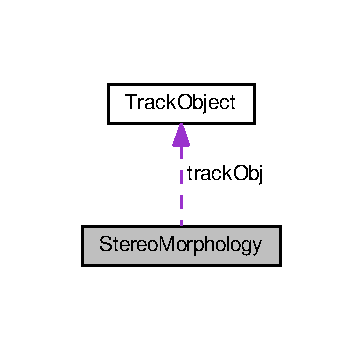
\includegraphics[width=174pt]{class_stereo_morphology__coll__graph}
\end{center}
\end{figure}
\subsection*{Public Member Functions}
\begin{DoxyCompactItemize}
\item 
void {\bfseries compute\+Overlay\+View} (Mat imageL, Mat disp\+\_\+\+B\+GR)\hypertarget{class_stereo_morphology_adb2fff0719a4b62a1c6e5752738fb80a}{}\label{class_stereo_morphology_adb2fff0719a4b62a1c6e5752738fb80a}

\item 
void {\bfseries compute\+Warning\+Edges\+View} ()\hypertarget{class_stereo_morphology_a0f47dff428aa0c6bfed3fdd732c0cda1}{}\label{class_stereo_morphology_a0f47dff428aa0c6bfed3fdd732c0cda1}

\item 
void \hyperlink{class_stereo_morphology_a553677016aadec1ee2e88554c7cb4c22}{apply\+Morphology} (Mat src, Mat tracking\+View, bool is\+Tracking\+Objects, int input\+Type, bool enable\+Lighting\+Noise\+Detector)
\item 
void {\bfseries apply\+\_\+pre\+Filtering} (Mat $\ast$src, Mat $\ast$dst)\hypertarget{class_stereo_morphology_a00905737b3af09a4bda72eb349b66cd2}{}\label{class_stereo_morphology_a00905737b3af09a4bda72eb349b66cd2}

\item 
void {\bfseries apply\+\_\+lighting\+Noise\+Detector} ()\hypertarget{class_stereo_morphology_a5f54239981aa543ba03b53a68dcd6942}{}\label{class_stereo_morphology_a5f54239981aa543ba03b53a68dcd6942}

\item 
void {\bfseries apply\+\_\+harris} (Mat src)\hypertarget{class_stereo_morphology_a1429831d7e87f2a21b4af5ddba7e2d0b}{}\label{class_stereo_morphology_a1429831d7e87f2a21b4af5ddba7e2d0b}

\item 
void \hyperlink{class_stereo_morphology_a238d8a135ab855a9acfeb6486fb799af}{apply\+\_\+watershed} (Mat src)
\begin{DoxyCompactList}\small\item\em Sample code showing how to segment overlapping objects using Laplacian filtering, in addition to Watershed and Distance Transformation. \end{DoxyCompactList}\item 
void {\bfseries Disp\+\_\+diff} (Mat disp8U, Mat disp8\+U\+\_\+last, Mat disp8\+U\+\_\+diff)\hypertarget{class_stereo_morphology_a0e3379db4ff0dde2c0e70c76cd34c0b3}{}\label{class_stereo_morphology_a0e3379db4ff0dde2c0e70c76cd34c0b3}

\end{DoxyCompactItemize}
\subsection*{Public Attributes}
\begin{DoxyCompactItemize}
\item 
\hyperlink{class_track_object}{Track\+Object} {\bfseries track\+Obj}\hypertarget{class_stereo_morphology_a7f6b936d970e28c9422e398dd6c79d17}{}\label{class_stereo_morphology_a7f6b936d970e28c9422e398dd6c79d17}

\item 
Mat {\bfseries disp\+B\+G\+R\+\_\+\+Filtered}\hypertarget{class_stereo_morphology_a806eb96195c81723df3d3fbded5be967}{}\label{class_stereo_morphology_a806eb96195c81723df3d3fbded5be967}

\item 
Mat {\bfseries disp\+\_\+\+B\+G\+R\+\_\+channels} \mbox{[}3\mbox{]}\hypertarget{class_stereo_morphology_a58993fc6b046e6b12287ba23794b7c3f}{}\label{class_stereo_morphology_a58993fc6b046e6b12287ba23794b7c3f}

\item 
Mat {\bfseries erosion\+Element}\hypertarget{class_stereo_morphology_a6ef36f8ee637fa3a111aa3fad0215ed8}{}\label{class_stereo_morphology_a6ef36f8ee637fa3a111aa3fad0215ed8}

\item 
Mat {\bfseries dilation\+Element}\hypertarget{class_stereo_morphology_afaea05d62b495bc255b9a4f067ef1de9}{}\label{class_stereo_morphology_afaea05d62b495bc255b9a4f067ef1de9}

\item 
int {\bfseries x}\hypertarget{class_stereo_morphology_ad8c81d26fefabbd2f105e7f6815100e1}{}\label{class_stereo_morphology_ad8c81d26fefabbd2f105e7f6815100e1}

\item 
int {\bfseries y}\hypertarget{class_stereo_morphology_a69992e3892562c8491c29010108f1b2a}{}\label{class_stereo_morphology_a69992e3892562c8491c29010108f1b2a}

\item 
Mat {\bfseries img\+Threshold}\hypertarget{class_stereo_morphology_adfb95e244ba8bc7513fd8c8d7373cc17}{}\label{class_stereo_morphology_adfb95e244ba8bc7513fd8c8d7373cc17}

\item 
Mat {\bfseries img\+Threshold\+Draw}\hypertarget{class_stereo_morphology_a41b49a076d7a23fe88e820537c29f701}{}\label{class_stereo_morphology_a41b49a076d7a23fe88e820537c29f701}

\item 
Mat {\bfseries tracking\+View}\hypertarget{class_stereo_morphology_a3c80c94aa9bad98198e14ab4ccb3fa8a}{}\label{class_stereo_morphology_a3c80c94aa9bad98198e14ab4ccb3fa8a}

\item 
Mat {\bfseries overlay\+View}\hypertarget{class_stereo_morphology_afb5fac41d2a38407666f3d15ae694a7e}{}\label{class_stereo_morphology_afb5fac41d2a38407666f3d15ae694a7e}

\end{DoxyCompactItemize}


\subsection{Member Function Documentation}
\index{Stereo\+Morphology@{Stereo\+Morphology}!apply\+\_\+watershed@{apply\+\_\+watershed}}
\index{apply\+\_\+watershed@{apply\+\_\+watershed}!Stereo\+Morphology@{Stereo\+Morphology}}
\subsubsection[{\texorpdfstring{apply\+\_\+watershed(\+Mat src)}{apply\_watershed(Mat src)}}]{\setlength{\rightskip}{0pt plus 5cm}void Stereo\+Morphology\+::apply\+\_\+watershed (
\begin{DoxyParamCaption}
\item[{Mat}]{src}
\end{DoxyParamCaption}
)}\hypertarget{class_stereo_morphology_a238d8a135ab855a9acfeb6486fb799af}{}\label{class_stereo_morphology_a238d8a135ab855a9acfeb6486fb799af}


Sample code showing how to segment overlapping objects using Laplacian filtering, in addition to Watershed and Distance Transformation. 

Watershed\+\_\+and\+\_\+\+Distance\+\_\+\+Transform.\+cpp \begin{DoxyAuthor}{Author}
Open\+CV Team 
\end{DoxyAuthor}
\mbox{[}load\+\_\+image\mbox{]}

\mbox{[}load\+\_\+image\mbox{]}

\mbox{[}black\+\_\+bg\mbox{]}

\mbox{[}black\+\_\+bg\mbox{]}

\mbox{[}sharp\mbox{]}

\mbox{[}sharp\mbox{]}

\mbox{[}bin\mbox{]}

\mbox{[}bin\mbox{]}

\mbox{[}dist\mbox{]}

\mbox{[}dist\mbox{]}

\mbox{[}peaks\mbox{]}

\mbox{[}peaks\mbox{]}

\mbox{[}seeds\mbox{]}

\mbox{[}seeds\mbox{]}

\mbox{[}watershed\mbox{]}

\mbox{[}watershed\mbox{]} \index{Stereo\+Morphology@{Stereo\+Morphology}!apply\+Morphology@{apply\+Morphology}}
\index{apply\+Morphology@{apply\+Morphology}!Stereo\+Morphology@{Stereo\+Morphology}}
\subsubsection[{\texorpdfstring{apply\+Morphology(\+Mat src, Mat tracking\+View, bool is\+Tracking\+Objects, int input\+Type, bool enable\+Lighting\+Noise\+Detector)}{applyMorphology(Mat src, Mat trackingView, bool isTrackingObjects, int inputType, bool enableLightingNoiseDetector)}}]{\setlength{\rightskip}{0pt plus 5cm}void Stereo\+Morphology\+::apply\+Morphology (
\begin{DoxyParamCaption}
\item[{Mat}]{src, }
\item[{Mat}]{tracking\+View, }
\item[{bool}]{is\+Tracking\+Objects, }
\item[{int}]{input\+Type, }
\item[{bool}]{enable\+Lighting\+Noise\+Detector}
\end{DoxyParamCaption}
)}\hypertarget{class_stereo_morphology_a553677016aadec1ee2e88554c7cb4c22}{}\label{class_stereo_morphology_a553677016aadec1ee2e88554c7cb4c22}
Near Object Detection !//

Testing Methods !//

Testing Blobs !// 

The documentation for this class was generated from the following files\+:\begin{DoxyCompactItemize}
\item 
inc/Stereo\+Morphology.\+h\item 
src/Stereo\+Morphology.\+cpp\end{DoxyCompactItemize}

\hypertarget{class_stereo_processor}{}\section{Stereo\+Processor Class Reference}
\label{class_stereo_processor}\index{Stereo\+Processor@{Stereo\+Processor}}


Inheritance diagram for Stereo\+Processor\+:
\nopagebreak
\begin{figure}[H]
\begin{center}
\leavevmode
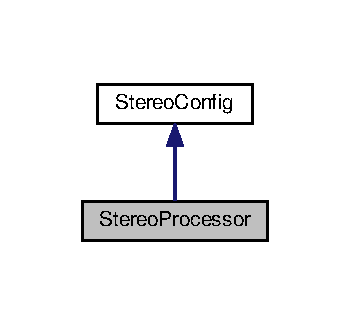
\includegraphics[width=168pt]{class_stereo_processor__inherit__graph}
\end{center}
\end{figure}


Collaboration diagram for Stereo\+Processor\+:
\nopagebreak
\begin{figure}[H]
\begin{center}
\leavevmode
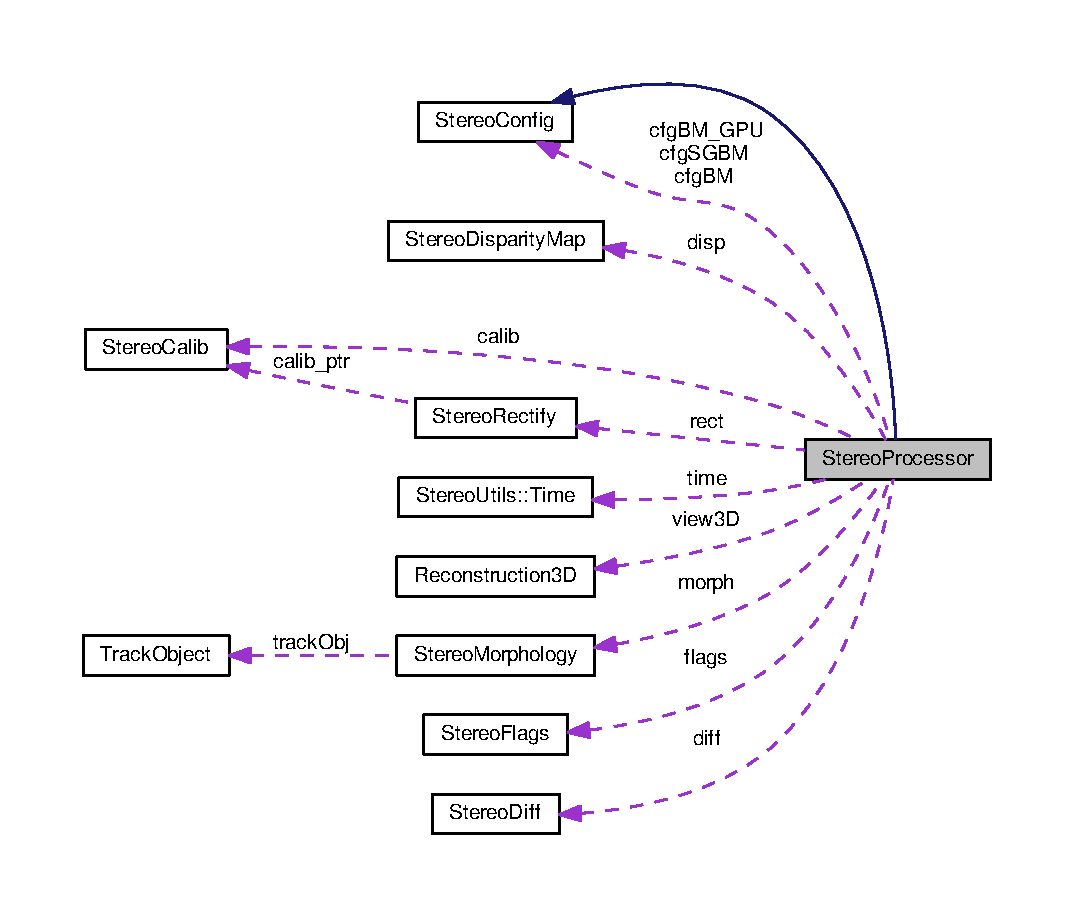
\includegraphics[width=350pt]{class_stereo_processor__coll__graph}
\end{center}
\end{figure}
\subsection*{Public Types}
\begin{DoxyCompactItemize}
\item 
enum \{ {\bfseries BM}, 
{\bfseries S\+G\+BM}, 
{\bfseries B\+M\+\_\+\+G\+PU}
 \}\hypertarget{class_stereo_processor_ad2d7c38c58a749e87183b5d7cd95e5f2}{}\label{class_stereo_processor_ad2d7c38c58a749e87183b5d7cd95e5f2}

\end{DoxyCompactItemize}
\subsection*{Public Member Functions}
\begin{DoxyCompactItemize}
\item 
{\bfseries Stereo\+Processor} (int input\+Num)\hypertarget{class_stereo_processor_ad7943f2a7d76a753bc006240b1fcf0f8}{}\label{class_stereo_processor_ad7943f2a7d76a753bc006240b1fcf0f8}

\item 
int {\bfseries get\+Input\+Num} ()\hypertarget{class_stereo_processor_a70b148471e8f97239a3523f35555664b}{}\label{class_stereo_processor_a70b148471e8f97239a3523f35555664b}

\item 
void {\bfseries read\+Config\+File} ()\hypertarget{class_stereo_processor_aac067ad8f9d37b32125679716e2747af}{}\label{class_stereo_processor_aac067ad8f9d37b32125679716e2747af}

\item 
void {\bfseries read\+Stereo\+B\+M\+Config\+File} ()\hypertarget{class_stereo_processor_ad3b8520e5fac5e91e7753ccb84cc42a5}{}\label{class_stereo_processor_ad3b8520e5fac5e91e7753ccb84cc42a5}

\item 
void {\bfseries read\+Stereo\+S\+G\+B\+M\+Config\+File} ()\hypertarget{class_stereo_processor_a3f1602fd35574e632448ac441795d6d1}{}\label{class_stereo_processor_a3f1602fd35574e632448ac441795d6d1}

\item 
void {\bfseries read\+Stereo\+B\+M\+\_\+\+G\+P\+U\+Config\+File} ()\hypertarget{class_stereo_processor_aae81bd7c15af3392286fcf8291c15839}{}\label{class_stereo_processor_aae81bd7c15af3392286fcf8291c15839}

\item 
void {\bfseries stereo\+B\+M\+\_\+\+Init} ()\hypertarget{class_stereo_processor_a4d3a0da0bc39fe82fcf964859acd7ced}{}\label{class_stereo_processor_a4d3a0da0bc39fe82fcf964859acd7ced}

\item 
void {\bfseries stereo\+S\+G\+B\+M\+\_\+\+Init} ()\hypertarget{class_stereo_processor_a27120807b020f1a1f3dab9f481172fc7}{}\label{class_stereo_processor_a27120807b020f1a1f3dab9f481172fc7}

\item 
void {\bfseries stereo\+B\+M\+\_\+\+G\+P\+U\+\_\+\+Init} ()\hypertarget{class_stereo_processor_aeffa85470ecc94865ce0943f4bf7920b}{}\label{class_stereo_processor_aeffa85470ecc94865ce0943f4bf7920b}

\item 
void {\bfseries set\+Stereo\+B\+M\+\_\+\+Params} ()\hypertarget{class_stereo_processor_a7544e7f43dfe9c90638b37800e3a7e86}{}\label{class_stereo_processor_a7544e7f43dfe9c90638b37800e3a7e86}

\item 
void {\bfseries set\+Stereo\+S\+G\+B\+M\+\_\+\+Params} ()\hypertarget{class_stereo_processor_a74da91a7bde48dd130b96a4c89b2cd6d}{}\label{class_stereo_processor_a74da91a7bde48dd130b96a4c89b2cd6d}

\item 
void {\bfseries set\+Stereo\+B\+M\+\_\+\+G\+P\+U\+\_\+\+Params} ()\hypertarget{class_stereo_processor_a65e413dd50eb5d08e7c2cf8552eabda9}{}\label{class_stereo_processor_a65e413dd50eb5d08e7c2cf8552eabda9}

\item 
void {\bfseries set\+Values} (int pre\+Filter\+Size, int pre\+Filter\+Cap, int sad\+Window\+Size, int min\+Disparity, int num\+Of\+Disparities, int texture\+Threshold, int uniqueness\+Ratio, int speckle\+Window\+Size, int speckle\+Window\+Range, int disp12\+Max\+Diff)\hypertarget{class_stereo_processor_a91a6b4bd83ca05386ce0c678f843344c}{}\label{class_stereo_processor_a91a6b4bd83ca05386ce0c678f843344c}

\item 
void {\bfseries set\+Num\+Rows} (int value)\hypertarget{class_stereo_processor_aac8a1975b0cb099516e14fca10db9ce3}{}\label{class_stereo_processor_aac8a1975b0cb099516e14fca10db9ce3}

\item 
void {\bfseries set\+Num\+Channels} (int value)\hypertarget{class_stereo_processor_a53ed33791c1d8ff5b7ea40cb06129d36}{}\label{class_stereo_processor_a53ed33791c1d8ff5b7ea40cb06129d36}

\item 
int {\bfseries get\+Num\+Rows} ()\hypertarget{class_stereo_processor_ac0d394ba023dd18613ad67cd635c954d}{}\label{class_stereo_processor_ac0d394ba023dd18613ad67cd635c954d}

\item 
int {\bfseries get\+Num\+Channels} ()\hypertarget{class_stereo_processor_ab988b47858da7462e01688284181d8f8}{}\label{class_stereo_processor_ab988b47858da7462e01688284181d8f8}

\item 
void {\bfseries capture\+Frames} ()\hypertarget{class_stereo_processor_ae4fc5d798217853b7ca317ad05922d91}{}\label{class_stereo_processor_ae4fc5d798217853b7ca317ad05922d91}

\item 
void \hyperlink{class_stereo_processor_a7e902a6a9ace8ba95aa42578f90bb5af}{calculate\+Disparities} ()
\item 
void {\bfseries calculate\+True\+Map} ()\hypertarget{class_stereo_processor_a467661ef75e0bcd07814500fc023beaf}{}\label{class_stereo_processor_a467661ef75e0bcd07814500fc023beaf}

\item 
void {\bfseries calculate3\+D\+Reconstruction} ()\hypertarget{class_stereo_processor_a00b4763b0e09947cef0a6f980bc3748a}{}\label{class_stereo_processor_a00b4763b0e09947cef0a6f980bc3748a}

\item 
void {\bfseries save\+Last\+Frames} ()\hypertarget{class_stereo_processor_afe313b6d97e8b1908cc65125042b2ec6}{}\label{class_stereo_processor_afe313b6d97e8b1908cc65125042b2ec6}

\item 
void {\bfseries video\+Looper} ()\hypertarget{class_stereo_processor_a30e7cd72b174b4dec0e2e34043446857}{}\label{class_stereo_processor_a30e7cd72b174b4dec0e2e34043446857}

\end{DoxyCompactItemize}
\subsection*{Public Attributes}
\begin{DoxyCompactItemize}
\item 
Mat {\bfseries imageL} \mbox{[}2\mbox{]}\hypertarget{class_stereo_processor_a352e81dcf5fcca68c82a6ce073d1b49e}{}\label{class_stereo_processor_a352e81dcf5fcca68c82a6ce073d1b49e}

\item 
Mat {\bfseries imageR} \mbox{[}2\mbox{]}\hypertarget{class_stereo_processor_abcaf44f4f9946757b64e574fd1a9fb5e}{}\label{class_stereo_processor_abcaf44f4f9946757b64e574fd1a9fb5e}

\item 
cuda\+::\+Gpu\+Mat {\bfseries d\+\_\+imageL}\hypertarget{class_stereo_processor_aa51dd141a845e61af77b3c1f7dbc65eb}{}\label{class_stereo_processor_aa51dd141a845e61af77b3c1f7dbc65eb}

\item 
cuda\+::\+Gpu\+Mat {\bfseries d\+\_\+imageR}\hypertarget{class_stereo_processor_aad3b42de5eaadb62cb5eda9ab76b187f}{}\label{class_stereo_processor_aad3b42de5eaadb62cb5eda9ab76b187f}

\item 
cuda\+::\+Gpu\+Mat {\bfseries d\+\_\+disp\+\_\+16S}\hypertarget{class_stereo_processor_a896676b5b447ef844d7372008f09d673}{}\label{class_stereo_processor_a896676b5b447ef844d7372008f09d673}

\item 
Mat {\bfseries image\+L\+\_\+grey} \mbox{[}2\mbox{]}\hypertarget{class_stereo_processor_acac50c2b80afaa42ce30d8e52e3138bc}{}\label{class_stereo_processor_acac50c2b80afaa42ce30d8e52e3138bc}

\item 
Mat {\bfseries image\+R\+\_\+grey} \mbox{[}2\mbox{]}\hypertarget{class_stereo_processor_a4883694b5935ae8f2a452d6f4690e743}{}\label{class_stereo_processor_a4883694b5935ae8f2a452d6f4690e743}

\item 
Video\+Capture {\bfseries capL}\hypertarget{class_stereo_processor_a3ba08a1fd4d6e4ec0eddf40fe75db779}{}\label{class_stereo_processor_a3ba08a1fd4d6e4ec0eddf40fe75db779}

\item 
Video\+Capture {\bfseries capR}\hypertarget{class_stereo_processor_afd4935a120da2d72c3e36a7f74ac0803}{}\label{class_stereo_processor_afd4935a120da2d72c3e36a7f74ac0803}

\item 
Ptr$<$ Stereo\+BM $>$ {\bfseries bm}\hypertarget{class_stereo_processor_a4299ddd0fa1226c8f881ff79c578cb92}{}\label{class_stereo_processor_a4299ddd0fa1226c8f881ff79c578cb92}

\item 
\hyperlink{class_stereo_config}{Stereo\+Config} {\bfseries cfg\+BM}\hypertarget{class_stereo_processor_acd131331e511be5ed98ee9016e241c89}{}\label{class_stereo_processor_acd131331e511be5ed98ee9016e241c89}

\item 
Ptr$<$ Stereo\+S\+G\+BM $>$ {\bfseries sgbm}\hypertarget{class_stereo_processor_a9ae4a559601753bb774fc85bb0fa4612}{}\label{class_stereo_processor_a9ae4a559601753bb774fc85bb0fa4612}

\item 
\hyperlink{class_stereo_config}{Stereo\+Config} {\bfseries cfg\+S\+G\+BM}\hypertarget{class_stereo_processor_a06957313554529ab5d1b0837020fe0c6}{}\label{class_stereo_processor_a06957313554529ab5d1b0837020fe0c6}

\item 
Ptr$<$ cuda\+::\+Stereo\+BM $>$ {\bfseries bm\+\_\+gpu}\hypertarget{class_stereo_processor_aee0fed0ac5c11a1b3fd3637658d124d5}{}\label{class_stereo_processor_aee0fed0ac5c11a1b3fd3637658d124d5}

\item 
\hyperlink{class_stereo_config}{Stereo\+Config} {\bfseries cfg\+B\+M\+\_\+\+G\+PU}\hypertarget{class_stereo_processor_a32e1ab4fd5a832446e3a8e0d9c26353b}{}\label{class_stereo_processor_a32e1ab4fd5a832446e3a8e0d9c26353b}

\item 
enum Stereo\+Processor\+:: \{ ... \}  {\bfseries method}\hypertarget{class_stereo_processor_a709a81b3a4f847479461350daeedc220}{}\label{class_stereo_processor_a709a81b3a4f847479461350daeedc220}

\item 
\hyperlink{class_stereo_calib}{Stereo\+Calib} {\bfseries calib}\hypertarget{class_stereo_processor_a6da4e21c22fa613fb225520cc1b80dd7}{}\label{class_stereo_processor_a6da4e21c22fa613fb225520cc1b80dd7}

\item 
\hyperlink{class_stereo_rectify}{Stereo\+Rectify} {\bfseries rect}\hypertarget{class_stereo_processor_a05398154b24291ad78ae80105005f9c1}{}\label{class_stereo_processor_a05398154b24291ad78ae80105005f9c1}

\item 
\hyperlink{class_stereo_disparity_map}{Stereo\+Disparity\+Map} {\bfseries disp}\hypertarget{class_stereo_processor_ad4790de5f5e466fd77b9737a06f01d76}{}\label{class_stereo_processor_ad4790de5f5e466fd77b9737a06f01d76}

\item 
\hyperlink{class_reconstruction3_d}{Reconstruction3D} {\bfseries view3D}\hypertarget{class_stereo_processor_a7f8c7fe5174d8dc8b99c2dad65758cdd}{}\label{class_stereo_processor_a7f8c7fe5174d8dc8b99c2dad65758cdd}

\item 
\hyperlink{class_stereo_diff}{Stereo\+Diff} {\bfseries diff}\hypertarget{class_stereo_processor_ad478da46fc5ab3ceac829165c838c864}{}\label{class_stereo_processor_ad478da46fc5ab3ceac829165c838c864}

\item 
\hyperlink{class_stereo_flags}{Stereo\+Flags} {\bfseries flags}\hypertarget{class_stereo_processor_a73e03785c78e6ab79d6d8951378a29ed}{}\label{class_stereo_processor_a73e03785c78e6ab79d6d8951378a29ed}

\item 
\hyperlink{class_stereo_utils_1_1_time}{Stereo\+Utils\+::\+Time} {\bfseries time}\hypertarget{class_stereo_processor_af8c3d91de1990ce04e4c5d6f49c5c37e}{}\label{class_stereo_processor_af8c3d91de1990ce04e4c5d6f49c5c37e}

\item 
\hyperlink{class_stereo_morphology}{Stereo\+Morphology} {\bfseries morph}\hypertarget{class_stereo_processor_a76bd7c120eb2ed266d69717bdb6d5aa6}{}\label{class_stereo_processor_a76bd7c120eb2ed266d69717bdb6d5aa6}

\item 
int {\bfseries frame\+Counter}\hypertarget{class_stereo_processor_ad33af3a32f3b3e1b9c1e0a9b6a7e5f0a}{}\label{class_stereo_processor_ad33af3a32f3b3e1b9c1e0a9b6a7e5f0a}

\item 
int {\bfseries x}\hypertarget{class_stereo_processor_a2afa82e29b04e9d3718f6fef951aea28}{}\label{class_stereo_processor_a2afa82e29b04e9d3718f6fef951aea28}

\item 
int {\bfseries y}\hypertarget{class_stereo_processor_a6b05bbc10ad304546804682d9aaa92ad}{}\label{class_stereo_processor_a6b05bbc10ad304546804682d9aaa92ad}

\item 
Mat {\bfseries true\+\_\+dmap}\hypertarget{class_stereo_processor_aa40150970588c5cbe44e890fdf51a86f}{}\label{class_stereo_processor_aa40150970588c5cbe44e890fdf51a86f}

\end{DoxyCompactItemize}


\subsection{Member Function Documentation}
\index{Stereo\+Processor@{Stereo\+Processor}!calculate\+Disparities@{calculate\+Disparities}}
\index{calculate\+Disparities@{calculate\+Disparities}!Stereo\+Processor@{Stereo\+Processor}}
\subsubsection[{\texorpdfstring{calculate\+Disparities()}{calculateDisparities()}}]{\setlength{\rightskip}{0pt plus 5cm}void Stereo\+Processor\+::calculate\+Disparities (
\begin{DoxyParamCaption}
{}
\end{DoxyParamCaption}
)}\hypertarget{class_stereo_processor_a7e902a6a9ace8ba95aa42578f90bb5af}{}\label{class_stereo_processor_a7e902a6a9ace8ba95aa42578f90bb5af}
S\+T\+A\+RT C\+L\+O\+CK !//

S\+T\+OP C\+L\+O\+CK !// 

The documentation for this class was generated from the following files\+:\begin{DoxyCompactItemize}
\item 
inc/Stereo\+Processor.\+h\item 
src/Stereo\+Processor.\+cpp\end{DoxyCompactItemize}

\hypertarget{class_stereo_rectify}{}\section{Stereo\+Rectify Class Reference}
\label{class_stereo_rectify}\index{Stereo\+Rectify@{Stereo\+Rectify}}


Collaboration diagram for Stereo\+Rectify\+:
\nopagebreak
\begin{figure}[H]
\begin{center}
\leavevmode
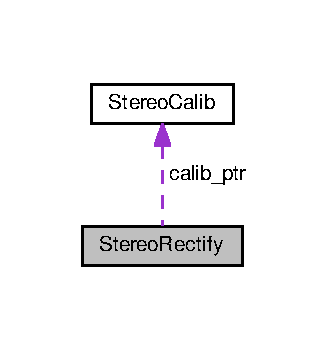
\includegraphics[width=158pt]{class_stereo_rectify__coll__graph}
\end{center}
\end{figure}
\subsection*{Public Member Functions}
\begin{DoxyCompactItemize}
\item 
{\bfseries Stereo\+Rectify} (\hyperlink{class_stereo_calib}{Stereo\+Calib} $\ast$ptr, Mat $\ast$ptrL, Mat $\ast$ptrR)\hypertarget{class_stereo_rectify_aed135d14152045de85f94bbac897abbd}{}\label{class_stereo_rectify_aed135d14152045de85f94bbac897abbd}

\item 
void {\bfseries init\+Rectification} ()\hypertarget{class_stereo_rectify_a257b2a3103f32c3fc305e0a49f7a246b}{}\label{class_stereo_rectify_a257b2a3103f32c3fc305e0a49f7a246b}

\item 
void \hyperlink{class_stereo_rectify_ab30b0c556bc470fdcc1c672ade8bcf50}{apply\+Rectification} ()
\item 
Mat {\bfseries get\+Image\+Lr} ()\hypertarget{class_stereo_rectify_ac92b1d24352fb5c4208574c2a1528ec8}{}\label{class_stereo_rectify_ac92b1d24352fb5c4208574c2a1528ec8}

\item 
Mat {\bfseries get\+Image\+Rr} ()\hypertarget{class_stereo_rectify_a1f9abe1a2b245ee51fd5844810e85b83}{}\label{class_stereo_rectify_a1f9abe1a2b245ee51fd5844810e85b83}

\end{DoxyCompactItemize}
\subsection*{Public Attributes}
\begin{DoxyCompactItemize}
\item 
\hyperlink{class_stereo_calib}{Stereo\+Calib} $\ast$ {\bfseries calib\+\_\+ptr}\hypertarget{class_stereo_rectify_a239c33a6951cd35c1ac14bad887f3aeb}{}\label{class_stereo_rectify_a239c33a6951cd35c1ac14bad887f3aeb}

\item 
Mat $\ast$ {\bfseries image\+L\+\_\+ptr}\hypertarget{class_stereo_rectify_a991cbbd311edb0f921cec0d835fc92ea}{}\label{class_stereo_rectify_a991cbbd311edb0f921cec0d835fc92ea}

\item 
Mat $\ast$ {\bfseries image\+R\+\_\+ptr}\hypertarget{class_stereo_rectify_ab9f6de69df67791f800a57acc4464969}{}\label{class_stereo_rectify_ab9f6de69df67791f800a57acc4464969}

\end{DoxyCompactItemize}


\subsection{Member Function Documentation}
\index{Stereo\+Rectify@{Stereo\+Rectify}!apply\+Rectification@{apply\+Rectification}}
\index{apply\+Rectification@{apply\+Rectification}!Stereo\+Rectify@{Stereo\+Rectify}}
\subsubsection[{\texorpdfstring{apply\+Rectification()}{applyRectification()}}]{\setlength{\rightskip}{0pt plus 5cm}void Stereo\+Rectify\+::apply\+Rectification (
\begin{DoxyParamCaption}
{}
\end{DoxyParamCaption}
)}\hypertarget{class_stereo_rectify_ab30b0c556bc470fdcc1c672ade8bcf50}{}\label{class_stereo_rectify_ab30b0c556bc470fdcc1c672ade8bcf50}
Do remapping of imageL to image\+Lr using map11, map12

Do remapping of imageR to image\+Rr using map21, map22 

The documentation for this class was generated from the following files\+:\begin{DoxyCompactItemize}
\item 
inc/Stereo\+Rectify.\+h\item 
src/Stereo\+Rectify.\+cpp\end{DoxyCompactItemize}

\hypertarget{class_stereo_utils_1_1_time}{}\section{Stereo\+Utils\+:\+:Time Class Reference}
\label{class_stereo_utils_1_1_time}\index{Stereo\+Utils\+::\+Time@{Stereo\+Utils\+::\+Time}}
\subsection*{Public Member Functions}
\begin{DoxyCompactItemize}
\item 
void {\bfseries calculate\+F\+PS} ()\hypertarget{class_stereo_utils_1_1_time_a73878c0fe0d43a42917e2f880e80c0d7}{}\label{class_stereo_utils_1_1_time_a73878c0fe0d43a42917e2f880e80c0d7}

\item 
void {\bfseries show\+F\+PS} ()\hypertarget{class_stereo_utils_1_1_time_a3ce678ed6e10245596b42550633b1fcd}{}\label{class_stereo_utils_1_1_time_a3ce678ed6e10245596b42550633b1fcd}

\item 
int {\bfseries get\+F\+PS} ()\hypertarget{class_stereo_utils_1_1_time_a805a1e98d58772c5f4f3bec4cfd3aeb4}{}\label{class_stereo_utils_1_1_time_a805a1e98d58772c5f4f3bec4cfd3aeb4}

\end{DoxyCompactItemize}
\subsection*{Static Public Member Functions}
\begin{DoxyCompactItemize}
\item 
static void {\bfseries start\+Clock} (int64 $\ast$initial)\hypertarget{class_stereo_utils_1_1_time_ad6a26260d6e34218f2f89484f47c6bb2}{}\label{class_stereo_utils_1_1_time_ad6a26260d6e34218f2f89484f47c6bb2}

\item 
static void {\bfseries stop\+Clock} (int64 $\ast$final)\hypertarget{class_stereo_utils_1_1_time_ae7d01a28068e42411b17de25ffa4717f}{}\label{class_stereo_utils_1_1_time_ae7d01a28068e42411b17de25ffa4717f}

\item 
static void {\bfseries print\+Elapsed\+Time} (int64 initial, int64 final)\hypertarget{class_stereo_utils_1_1_time_affb80835fb8675cf64b155471caa8fa3}{}\label{class_stereo_utils_1_1_time_affb80835fb8675cf64b155471caa8fa3}

\end{DoxyCompactItemize}
\subsection*{Public Attributes}
\begin{DoxyCompactItemize}
\item 
int64 {\bfseries clock\+Initial}\hypertarget{class_stereo_utils_1_1_time_aeee8c2529192336c91ee59e9a2a2d9d4}{}\label{class_stereo_utils_1_1_time_aeee8c2529192336c91ee59e9a2a2d9d4}

\item 
int64 {\bfseries clock\+Final}\hypertarget{class_stereo_utils_1_1_time_a36304edf947ce531a08fddab291cd90d}{}\label{class_stereo_utils_1_1_time_a36304edf947ce531a08fddab291cd90d}

\item 
int64 {\bfseries clock\+Initial\+\_\+d}\hypertarget{class_stereo_utils_1_1_time_a53d830a50f304c24adee4d005b329d07}{}\label{class_stereo_utils_1_1_time_a53d830a50f304c24adee4d005b329d07}

\item 
int64 {\bfseries clock\+Final\+\_\+d}\hypertarget{class_stereo_utils_1_1_time_af7658b229732620deee17078d388badb}{}\label{class_stereo_utils_1_1_time_af7658b229732620deee17078d388badb}

\item 
int64 {\bfseries d}\hypertarget{class_stereo_utils_1_1_time_aaf6dd4d4ebb54cf2ec93186fa36bd014}{}\label{class_stereo_utils_1_1_time_aaf6dd4d4ebb54cf2ec93186fa36bd014}

\item 
double {\bfseries f}\hypertarget{class_stereo_utils_1_1_time_a59464d8bf787a21394a72731b8fde1fa}{}\label{class_stereo_utils_1_1_time_a59464d8bf787a21394a72731b8fde1fa}

\end{DoxyCompactItemize}


The documentation for this class was generated from the following files\+:\begin{DoxyCompactItemize}
\item 
inc/Stereo\+Utils.\+h\item 
src/Stereo\+Utils.\+cpp\end{DoxyCompactItemize}

\hypertarget{class_track_object}{}\section{Track\+Object Class Reference}
\label{class_track_object}\index{Track\+Object@{Track\+Object}}
\subsection*{Public Member Functions}
\begin{DoxyCompactItemize}
\item 
void {\bfseries track\+Filtered\+Object} (int \&x, int \&y, Mat threshold, Mat \&camera\+Feed)\hypertarget{class_track_object_a47930962ed05342a7944e0983b44dcfd}{}\label{class_track_object_a47930962ed05342a7944e0983b44dcfd}

\item 
void {\bfseries draw\+Object} (int x, int y, Mat \&frame)\hypertarget{class_track_object_a46528f85400eb695f023de87e3eaa082}{}\label{class_track_object_a46528f85400eb695f023de87e3eaa082}

\item 
string {\bfseries int\+To\+String} (int number)\hypertarget{class_track_object_a7322039b592a9af2072c26963a9c843f}{}\label{class_track_object_a7322039b592a9af2072c26963a9c843f}

\end{DoxyCompactItemize}


The documentation for this class was generated from the following files\+:\begin{DoxyCompactItemize}
\item 
inc/track\+Object.\+h\item 
src/track\+Object.\+cpp\end{DoxyCompactItemize}

\hypertarget{class_ui___main_window}{}\section{Ui\+\_\+\+Main\+Window Class Reference}
\label{class_ui___main_window}\index{Ui\+\_\+\+Main\+Window@{Ui\+\_\+\+Main\+Window}}


Inheritance diagram for Ui\+\_\+\+Main\+Window\+:
\nopagebreak
\begin{figure}[H]
\begin{center}
\leavevmode
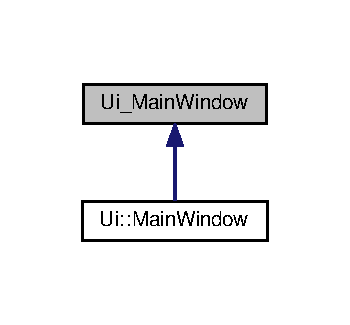
\includegraphics[width=168pt]{class_ui___main_window__inherit__graph}
\end{center}
\end{figure}
\subsection*{Public Member Functions}
\begin{DoxyCompactItemize}
\item 
void {\bfseries setup\+Ui} (Q\+Main\+Window $\ast$\hyperlink{class_main_window}{Main\+Window})\hypertarget{class_ui___main_window_acf4a0872c4c77d8f43a2ec66ed849b58}{}\label{class_ui___main_window_acf4a0872c4c77d8f43a2ec66ed849b58}

\item 
void {\bfseries retranslate\+Ui} (Q\+Main\+Window $\ast$\hyperlink{class_main_window}{Main\+Window})\hypertarget{class_ui___main_window_a097dd160c3534a204904cb374412c618}{}\label{class_ui___main_window_a097dd160c3534a204904cb374412c618}

\end{DoxyCompactItemize}
\subsection*{Public Attributes}
\begin{DoxyCompactItemize}
\item 
Q\+Widget $\ast$ {\bfseries central\+Widget}\hypertarget{class_ui___main_window_a30075506c2116c3ed4ff25e07ae75f81}{}\label{class_ui___main_window_a30075506c2116c3ed4ff25e07ae75f81}

\item 
Q\+Label $\ast$ {\bfseries lbl\+Original\+Left}\hypertarget{class_ui___main_window_a5337796623df84ca8de4d3664294f35e}{}\label{class_ui___main_window_a5337796623df84ca8de4d3664294f35e}

\item 
Q\+Label $\ast$ {\bfseries lbl\+Original\+Right}\hypertarget{class_ui___main_window_a189d3a7b1c5a9d2142cc56a4127ba57d}{}\label{class_ui___main_window_a189d3a7b1c5a9d2142cc56a4127ba57d}

\item 
Q\+Plain\+Text\+Edit $\ast$ {\bfseries text\+Box\+Output}\hypertarget{class_ui___main_window_a20ac574a2eebbef480a7bde5a46f1bbf}{}\label{class_ui___main_window_a20ac574a2eebbef480a7bde5a46f1bbf}

\item 
Q\+Push\+Button $\ast$ {\bfseries btn\+Pause\+Or\+Resume}\hypertarget{class_ui___main_window_a78f374f2f7411a6220b13d127451d341}{}\label{class_ui___main_window_a78f374f2f7411a6220b13d127451d341}

\item 
Q\+Push\+Button $\ast$ {\bfseries btn\+Show\+Disparity\+Map}\hypertarget{class_ui___main_window_aee6041a8cd86e1c236b7886d01c8a332}{}\label{class_ui___main_window_aee6041a8cd86e1c236b7886d01c8a332}

\item 
Q\+Push\+Button $\ast$ {\bfseries btn\+Show\+Stereo\+Param\+Setup}\hypertarget{class_ui___main_window_abbec93e8a58f0fba9a7e31ece8d83c4c}{}\label{class_ui___main_window_abbec93e8a58f0fba9a7e31ece8d83c4c}

\item 
Q\+Push\+Button $\ast$ {\bfseries btn\+Show3\+D\+Reconstruction}\hypertarget{class_ui___main_window_a59ef5ea36b7ee42a9a65b3c2c85f9e91}{}\label{class_ui___main_window_a59ef5ea36b7ee42a9a65b3c2c85f9e91}

\item 
Q\+Push\+Button $\ast$ {\bfseries btn\+Show\+Input\+Images}\hypertarget{class_ui___main_window_a460acfa3b85a277ff112d34d68b1d9fb}{}\label{class_ui___main_window_a460acfa3b85a277ff112d34d68b1d9fb}

\item 
Q\+Push\+Button $\ast$ {\bfseries btn\+Show\+Tracking\+Object\+View}\hypertarget{class_ui___main_window_a5826d8e6447af41ca3ed383217141e05}{}\label{class_ui___main_window_a5826d8e6447af41ca3ed383217141e05}

\item 
Q\+Push\+Button $\ast$ {\bfseries btn\+Show\+Diff\+Image}\hypertarget{class_ui___main_window_a0d0325ec82050a9de5d10d14f1589ad2}{}\label{class_ui___main_window_a0d0325ec82050a9de5d10d14f1589ad2}

\item 
Q\+Push\+Button $\ast$ {\bfseries btn\+Show\+Warning\+Lines}\hypertarget{class_ui___main_window_ad71edbfb8100c5bc2bc28ab926a4d426}{}\label{class_ui___main_window_ad71edbfb8100c5bc2bc28ab926a4d426}

\item 
Q\+Combo\+Box $\ast$ {\bfseries method\+Selector}\hypertarget{class_ui___main_window_a7dc757283ef86dae9c569ff9b309471d}{}\label{class_ui___main_window_a7dc757283ef86dae9c569ff9b309471d}

\item 
Q\+L\+C\+D\+Number $\ast$ {\bfseries lcd\+Number}\hypertarget{class_ui___main_window_aeaa664b636e02543a3047acb6d8918c5}{}\label{class_ui___main_window_aeaa664b636e02543a3047acb6d8918c5}

\item 
Q\+Push\+Button $\ast$ {\bfseries toggle\+Btn\+Show\+Hist}\hypertarget{class_ui___main_window_a21d86f2c5c275540e88c7389cae49de3}{}\label{class_ui___main_window_a21d86f2c5c275540e88c7389cae49de3}

\item 
Q\+Push\+Button $\ast$ {\bfseries toggle\+Btn\+Show\+X\+YZ}\hypertarget{class_ui___main_window_a88a4b46d267cadbaa69a3934abdbca88}{}\label{class_ui___main_window_a88a4b46d267cadbaa69a3934abdbca88}

\item 
Q\+Push\+Button $\ast$ {\bfseries toggle\+Btn\+Show\+Disp\+Depth}\hypertarget{class_ui___main_window_a858c2f497438654ce1613a9bf2505cc6}{}\label{class_ui___main_window_a858c2f497438654ce1613a9bf2505cc6}

\item 
Q\+Combo\+Box $\ast$ {\bfseries input\+Selector}\hypertarget{class_ui___main_window_aac393ae8df4601334b50ebf65d67ef9d}{}\label{class_ui___main_window_aac393ae8df4601334b50ebf65d67ef9d}

\item 
Q\+Push\+Button $\ast$ {\bfseries toggle\+Btn\+Show\+Left\+Image}\hypertarget{class_ui___main_window_ab46a543a56d143443d424cb611d205fd}{}\label{class_ui___main_window_ab46a543a56d143443d424cb611d205fd}

\item 
Q\+Push\+Button $\ast$ {\bfseries toggle\+Btn\+Show\+Overlay}\hypertarget{class_ui___main_window_a550e65cd07cfa9c1fd1f3f2bc000701c}{}\label{class_ui___main_window_a550e65cd07cfa9c1fd1f3f2bc000701c}

\item 
Q\+Menu\+Bar $\ast$ {\bfseries menu\+Bar}\hypertarget{class_ui___main_window_a2be1c24ec9adfca18e1dcc951931457f}{}\label{class_ui___main_window_a2be1c24ec9adfca18e1dcc951931457f}

\item 
Q\+Status\+Bar $\ast$ {\bfseries status\+Bar}\hypertarget{class_ui___main_window_a50fa481337604bcc8bf68de18ab16ecd}{}\label{class_ui___main_window_a50fa481337604bcc8bf68de18ab16ecd}

\end{DoxyCompactItemize}


The documentation for this class was generated from the following file\+:\begin{DoxyCompactItemize}
\item 
tmp/moc/ui\+\_\+mainwindow.\+h\end{DoxyCompactItemize}

\hypertarget{class_ui___set_stereo_params}{}\section{Ui\+\_\+\+Set\+Stereo\+Params Class Reference}
\label{class_ui___set_stereo_params}\index{Ui\+\_\+\+Set\+Stereo\+Params@{Ui\+\_\+\+Set\+Stereo\+Params}}


Inheritance diagram for Ui\+\_\+\+Set\+Stereo\+Params\+:
\nopagebreak
\begin{figure}[H]
\begin{center}
\leavevmode
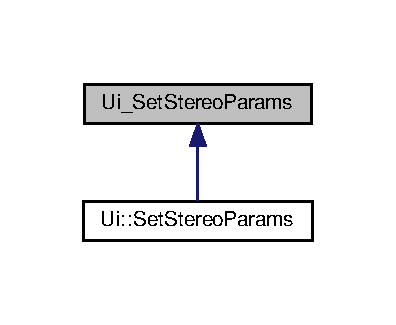
\includegraphics[width=190pt]{class_ui___set_stereo_params__inherit__graph}
\end{center}
\end{figure}
\subsection*{Public Member Functions}
\begin{DoxyCompactItemize}
\item 
void {\bfseries setup\+Ui} (Q\+Dialog $\ast$\hyperlink{class_set_stereo_params}{Set\+Stereo\+Params})\hypertarget{class_ui___set_stereo_params_a14abad600eb358910e00beda2062ce70}{}\label{class_ui___set_stereo_params_a14abad600eb358910e00beda2062ce70}

\item 
void {\bfseries retranslate\+Ui} (Q\+Dialog $\ast$\hyperlink{class_set_stereo_params}{Set\+Stereo\+Params})\hypertarget{class_ui___set_stereo_params_a10deece6ae48222b69698c6cf37d463a}{}\label{class_ui___set_stereo_params_a10deece6ae48222b69698c6cf37d463a}

\end{DoxyCompactItemize}
\subsection*{Public Attributes}
\begin{DoxyCompactItemize}
\item 
Q\+Dialog\+Button\+Box $\ast$ {\bfseries button\+Box}\hypertarget{class_ui___set_stereo_params_ad11244eef2b54d5027393f58eb902059}{}\label{class_ui___set_stereo_params_ad11244eef2b54d5027393f58eb902059}

\item 
Q\+Slider $\ast$ {\bfseries pre\+Filter\+Size\+\_\+slider}\hypertarget{class_ui___set_stereo_params_a9210a6deebe352f72a7a5b91d99f8d4b}{}\label{class_ui___set_stereo_params_a9210a6deebe352f72a7a5b91d99f8d4b}

\item 
Q\+Spin\+Box $\ast$ {\bfseries pre\+Filter\+Size\+\_\+spin\+Box}\hypertarget{class_ui___set_stereo_params_a9a49e09cc5c48ca4ff643f6bead80e53}{}\label{class_ui___set_stereo_params_a9a49e09cc5c48ca4ff643f6bead80e53}

\item 
Q\+Slider $\ast$ {\bfseries pre\+Filter\+Cap\+\_\+slider}\hypertarget{class_ui___set_stereo_params_a0b9f1a09a227d6e800f44dfa30804ede}{}\label{class_ui___set_stereo_params_a0b9f1a09a227d6e800f44dfa30804ede}

\item 
Q\+Spin\+Box $\ast$ {\bfseries pre\+Filter\+Cap\+\_\+spin\+Box}\hypertarget{class_ui___set_stereo_params_a47b596659bb042ae51a69c10a7444154}{}\label{class_ui___set_stereo_params_a47b596659bb042ae51a69c10a7444154}

\item 
Q\+Label $\ast$ {\bfseries pre\+Filter\+Size\+\_\+label}\hypertarget{class_ui___set_stereo_params_a7d2896335e056073279af1bc0ac7468e}{}\label{class_ui___set_stereo_params_a7d2896335e056073279af1bc0ac7468e}

\item 
Q\+Label $\ast$ {\bfseries pre\+Filter\+Cap\+\_\+label}\hypertarget{class_ui___set_stereo_params_a87361f774275294494d36556ce41b0e2}{}\label{class_ui___set_stereo_params_a87361f774275294494d36556ce41b0e2}

\item 
Q\+Label $\ast$ {\bfseries S\+A\+D\+Window\+Size\+\_\+label}\hypertarget{class_ui___set_stereo_params_aff0eaf3bda2cdfc0f8e745ada1671fbe}{}\label{class_ui___set_stereo_params_aff0eaf3bda2cdfc0f8e745ada1671fbe}

\item 
Q\+Slider $\ast$ {\bfseries S\+A\+D\+Window\+Size\+\_\+slider}\hypertarget{class_ui___set_stereo_params_afdd2000c79c0a6632fb0a28fd89de891}{}\label{class_ui___set_stereo_params_afdd2000c79c0a6632fb0a28fd89de891}

\item 
Q\+Spin\+Box $\ast$ {\bfseries S\+A\+D\+Window\+Size\+\_\+spin\+Box}\hypertarget{class_ui___set_stereo_params_ab3d195ceca7ddc46e18f912e8b5136a5}{}\label{class_ui___set_stereo_params_ab3d195ceca7ddc46e18f912e8b5136a5}

\item 
Q\+Label $\ast$ {\bfseries min\+Disparity\+\_\+label}\hypertarget{class_ui___set_stereo_params_a398506e059afe6317fac8349b10bc9c1}{}\label{class_ui___set_stereo_params_a398506e059afe6317fac8349b10bc9c1}

\item 
Q\+Slider $\ast$ {\bfseries min\+Disparity\+\_\+slider}\hypertarget{class_ui___set_stereo_params_a341c8eeec96c6f1555b46c17d392ffc3}{}\label{class_ui___set_stereo_params_a341c8eeec96c6f1555b46c17d392ffc3}

\item 
Q\+Spin\+Box $\ast$ {\bfseries min\+Disparity\+\_\+spin\+Box}\hypertarget{class_ui___set_stereo_params_abd4f8b95f839308df1e72e61eb0562f9}{}\label{class_ui___set_stereo_params_abd4f8b95f839308df1e72e61eb0562f9}

\item 
Q\+Label $\ast$ {\bfseries number\+Of\+Disparities\+\_\+label}\hypertarget{class_ui___set_stereo_params_a585df427da310e51698f41b509884d4a}{}\label{class_ui___set_stereo_params_a585df427da310e51698f41b509884d4a}

\item 
Q\+Slider $\ast$ {\bfseries number\+Of\+Disparities\+\_\+slider}\hypertarget{class_ui___set_stereo_params_afc362b6b668e0102a7adfb7c079206d7}{}\label{class_ui___set_stereo_params_afc362b6b668e0102a7adfb7c079206d7}

\item 
Q\+Spin\+Box $\ast$ {\bfseries number\+Of\+Disparities\+\_\+spin\+Box}\hypertarget{class_ui___set_stereo_params_aa4ab14f54a5a9522e519d4a559993625}{}\label{class_ui___set_stereo_params_aa4ab14f54a5a9522e519d4a559993625}

\item 
Q\+Label $\ast$ {\bfseries texture\+Threshold\+\_\+label}\hypertarget{class_ui___set_stereo_params_abbd73c97a65f3c4ebc9a50e4e7b59efa}{}\label{class_ui___set_stereo_params_abbd73c97a65f3c4ebc9a50e4e7b59efa}

\item 
Q\+Slider $\ast$ {\bfseries texture\+Threshold\+\_\+slider}\hypertarget{class_ui___set_stereo_params_a210bbddaed52a938c0320996f07ba509}{}\label{class_ui___set_stereo_params_a210bbddaed52a938c0320996f07ba509}

\item 
Q\+Spin\+Box $\ast$ {\bfseries texture\+Threshold\+\_\+spin\+Box}\hypertarget{class_ui___set_stereo_params_affe92fd3010e745187986e077856309f}{}\label{class_ui___set_stereo_params_affe92fd3010e745187986e077856309f}

\item 
Q\+Label $\ast$ {\bfseries uniqueness\+Ratio\+\_\+label}\hypertarget{class_ui___set_stereo_params_abc7acd67b2a18349dd575b039467b466}{}\label{class_ui___set_stereo_params_abc7acd67b2a18349dd575b039467b466}

\item 
Q\+Slider $\ast$ {\bfseries uniqueness\+Ratio\+\_\+slider}\hypertarget{class_ui___set_stereo_params_ad8a7ce981cb11a082072561b07bfa8e9}{}\label{class_ui___set_stereo_params_ad8a7ce981cb11a082072561b07bfa8e9}

\item 
Q\+Spin\+Box $\ast$ {\bfseries uniqueness\+Ratio\+\_\+spin\+Box}\hypertarget{class_ui___set_stereo_params_ad865475f3d02b22b7bd909cbf3817cd8}{}\label{class_ui___set_stereo_params_ad865475f3d02b22b7bd909cbf3817cd8}

\item 
Q\+Label $\ast$ {\bfseries speckle\+Window\+Size\+\_\+label}\hypertarget{class_ui___set_stereo_params_a07750305cb315bab77e5314c5448334c}{}\label{class_ui___set_stereo_params_a07750305cb315bab77e5314c5448334c}

\item 
Q\+Slider $\ast$ {\bfseries speckle\+Window\+Size\+\_\+slider}\hypertarget{class_ui___set_stereo_params_a89eb0366123c53fa25d797702b70eef3}{}\label{class_ui___set_stereo_params_a89eb0366123c53fa25d797702b70eef3}

\item 
Q\+Spin\+Box $\ast$ {\bfseries speckle\+Window\+Size\+\_\+spin\+Box}\hypertarget{class_ui___set_stereo_params_ab549c22969ede27596584fa0f496ae65}{}\label{class_ui___set_stereo_params_ab549c22969ede27596584fa0f496ae65}

\item 
Q\+Label $\ast$ {\bfseries speckle\+Range\+\_\+label}\hypertarget{class_ui___set_stereo_params_a83c8ba98034c5d8eea956c22474adc4f}{}\label{class_ui___set_stereo_params_a83c8ba98034c5d8eea956c22474adc4f}

\item 
Q\+Slider $\ast$ {\bfseries speckle\+Range\+\_\+slider}\hypertarget{class_ui___set_stereo_params_a61638a0d0a65f4e4a39b958e9452ee7d}{}\label{class_ui___set_stereo_params_a61638a0d0a65f4e4a39b958e9452ee7d}

\item 
Q\+Spin\+Box $\ast$ {\bfseries speckle\+Range\+\_\+spin\+Box}\hypertarget{class_ui___set_stereo_params_a7c4da87db1e119212bf3fd90b88d02f8}{}\label{class_ui___set_stereo_params_a7c4da87db1e119212bf3fd90b88d02f8}

\item 
Q\+Label $\ast$ {\bfseries disp12\+Max\+Diff\+\_\+label}\hypertarget{class_ui___set_stereo_params_a1fa58eb96e57c066cb98f1471d94bce2}{}\label{class_ui___set_stereo_params_a1fa58eb96e57c066cb98f1471d94bce2}

\item 
Q\+Slider $\ast$ {\bfseries disp12\+Max\+Diff\+\_\+slider}\hypertarget{class_ui___set_stereo_params_a6b7336ca20cecafe5c020efefe074a14}{}\label{class_ui___set_stereo_params_a6b7336ca20cecafe5c020efefe074a14}

\item 
Q\+Spin\+Box $\ast$ {\bfseries disp12\+Max\+Diff\+\_\+spin\+Box}\hypertarget{class_ui___set_stereo_params_a312f83936aab13a3d6fee7157f571cf8}{}\label{class_ui___set_stereo_params_a312f83936aab13a3d6fee7157f571cf8}

\end{DoxyCompactItemize}


The documentation for this class was generated from the following file\+:\begin{DoxyCompactItemize}
\item 
tmp/moc/ui\+\_\+setstereoparams.\+h\end{DoxyCompactItemize}

%--- End generated contents ---

% Index
\backmatter
\newpage
\phantomsection
\clearemptydoublepage
\addcontentsline{toc}{chapter}{Index}
\printindex

\end{document}
